\documentclass[13pt]{article}

\usepackage{url}
\usepackage{pstricks,pst-node,pst-text,pst-3d}
\usepackage{amsmath}
\usepackage{mathrsfs}
\usepackage{amssymb}
\usepackage{graphics}
\usepackage{epsfig}
\usepackage{fancyhdr}



\author{Brian Fehrman}
\title{Computer Vision Fall 2012: HW4 Pinhole Camera Write-Up}

\begin{document}
\maketitle

\section{Introduction}
This document is a short write up on my build process of a pinhole camera. My slight twist on this is that I used a webcam instead of a digital still camera or film paper to record the image. In addition to this, I did some processing on the recorded footage using OpenCV. The video file was read in, it was rotated to the correct orientation (180 degrees), and this corrected video was saved to a new file. Furthermore, I had OpenCV perform an SVD on the footage and create a new video which is the original footage but in a rank 5 representation (and is now in gray scale). Before processing could be done, the recorded footage was scaled down in resolution because my laptop just can't a large load. The FPS on the output videos are something that still needs to be tweaked. Included with this writeup are the original footage, the scaled footage, the rotated footage, and the lower rank representation of the footage.

\section{Materials}
The materials that were used are as follows:

\begin{enumerate}
\item A box
\item Black spray paint
\item White paper
\item Scotch tape
\item Electrical tape
\item Webcam
\item Duct tape
\item Tin foil
\item Velcro
\end{enumerate}

\section{The Build}


\begin{figure}[ht!]
\centering
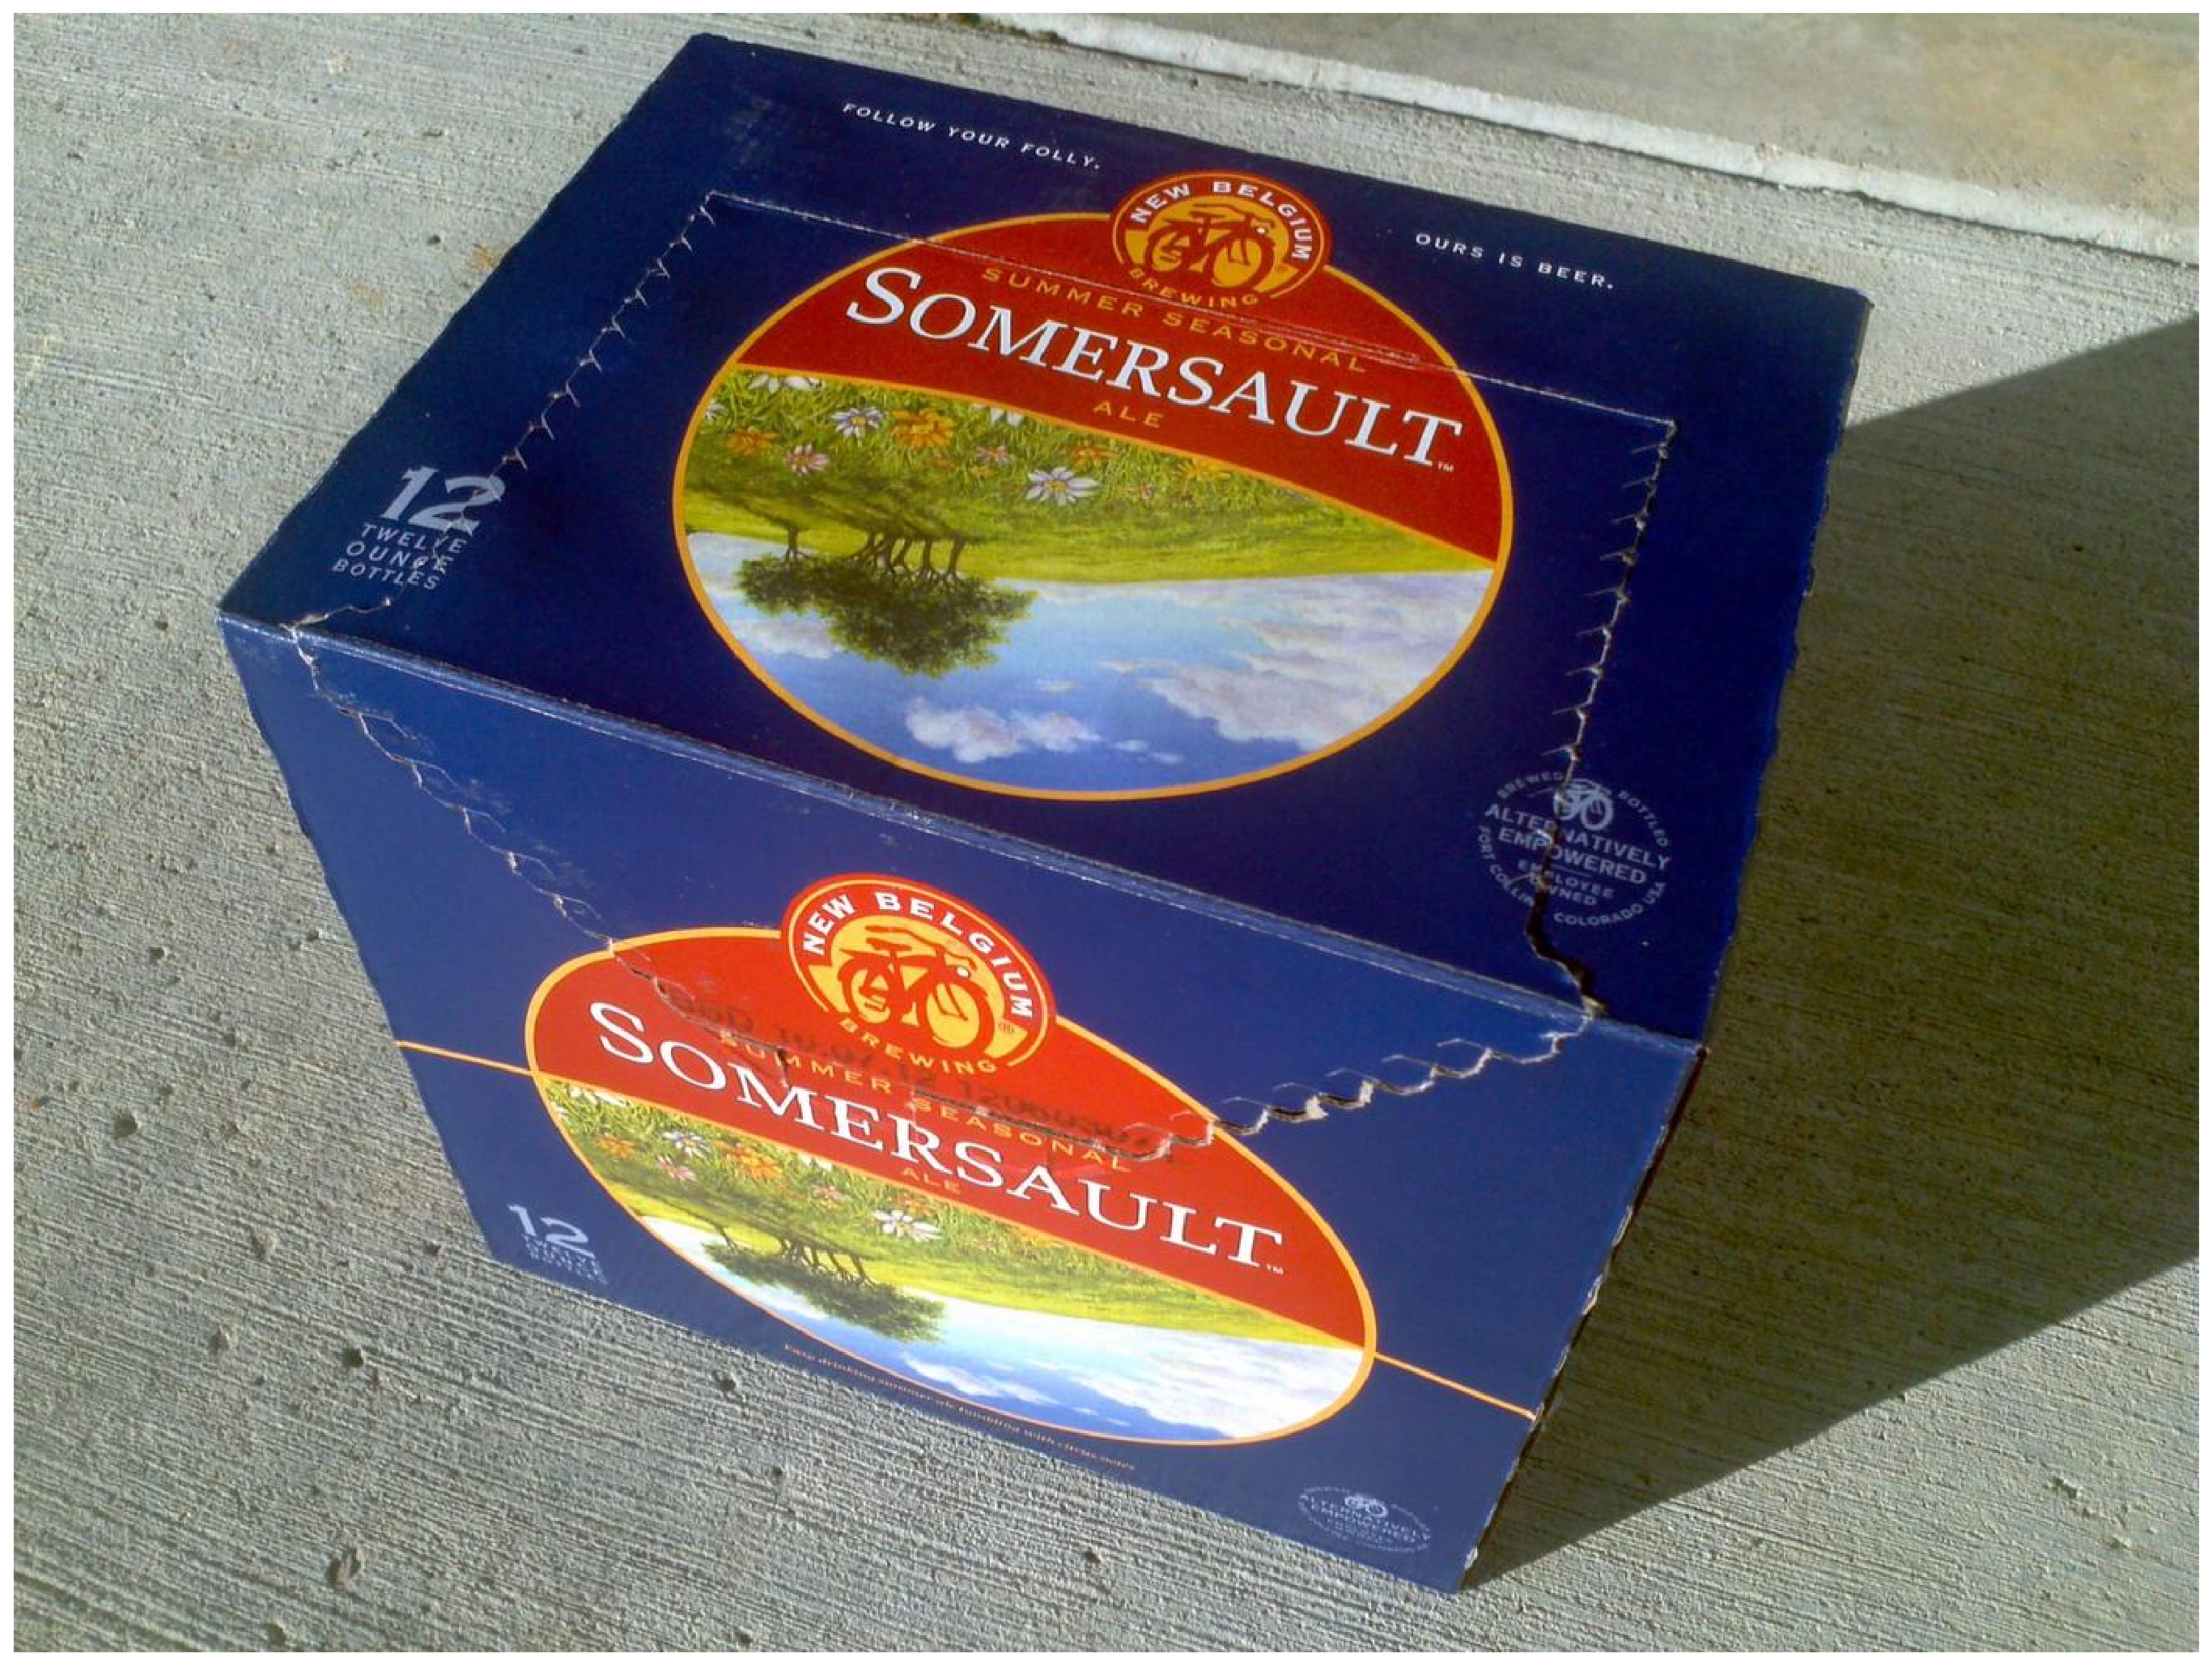
\includegraphics[width=0.8\textwidth]{eps/fullBox.eps}
\caption{First, find yourself a good sturdy box. If it is already fairly light tight then this is even better.
	 \label{fig:fullBox}} 
\end{figure}

\begin{figure}[ht!]
\centering
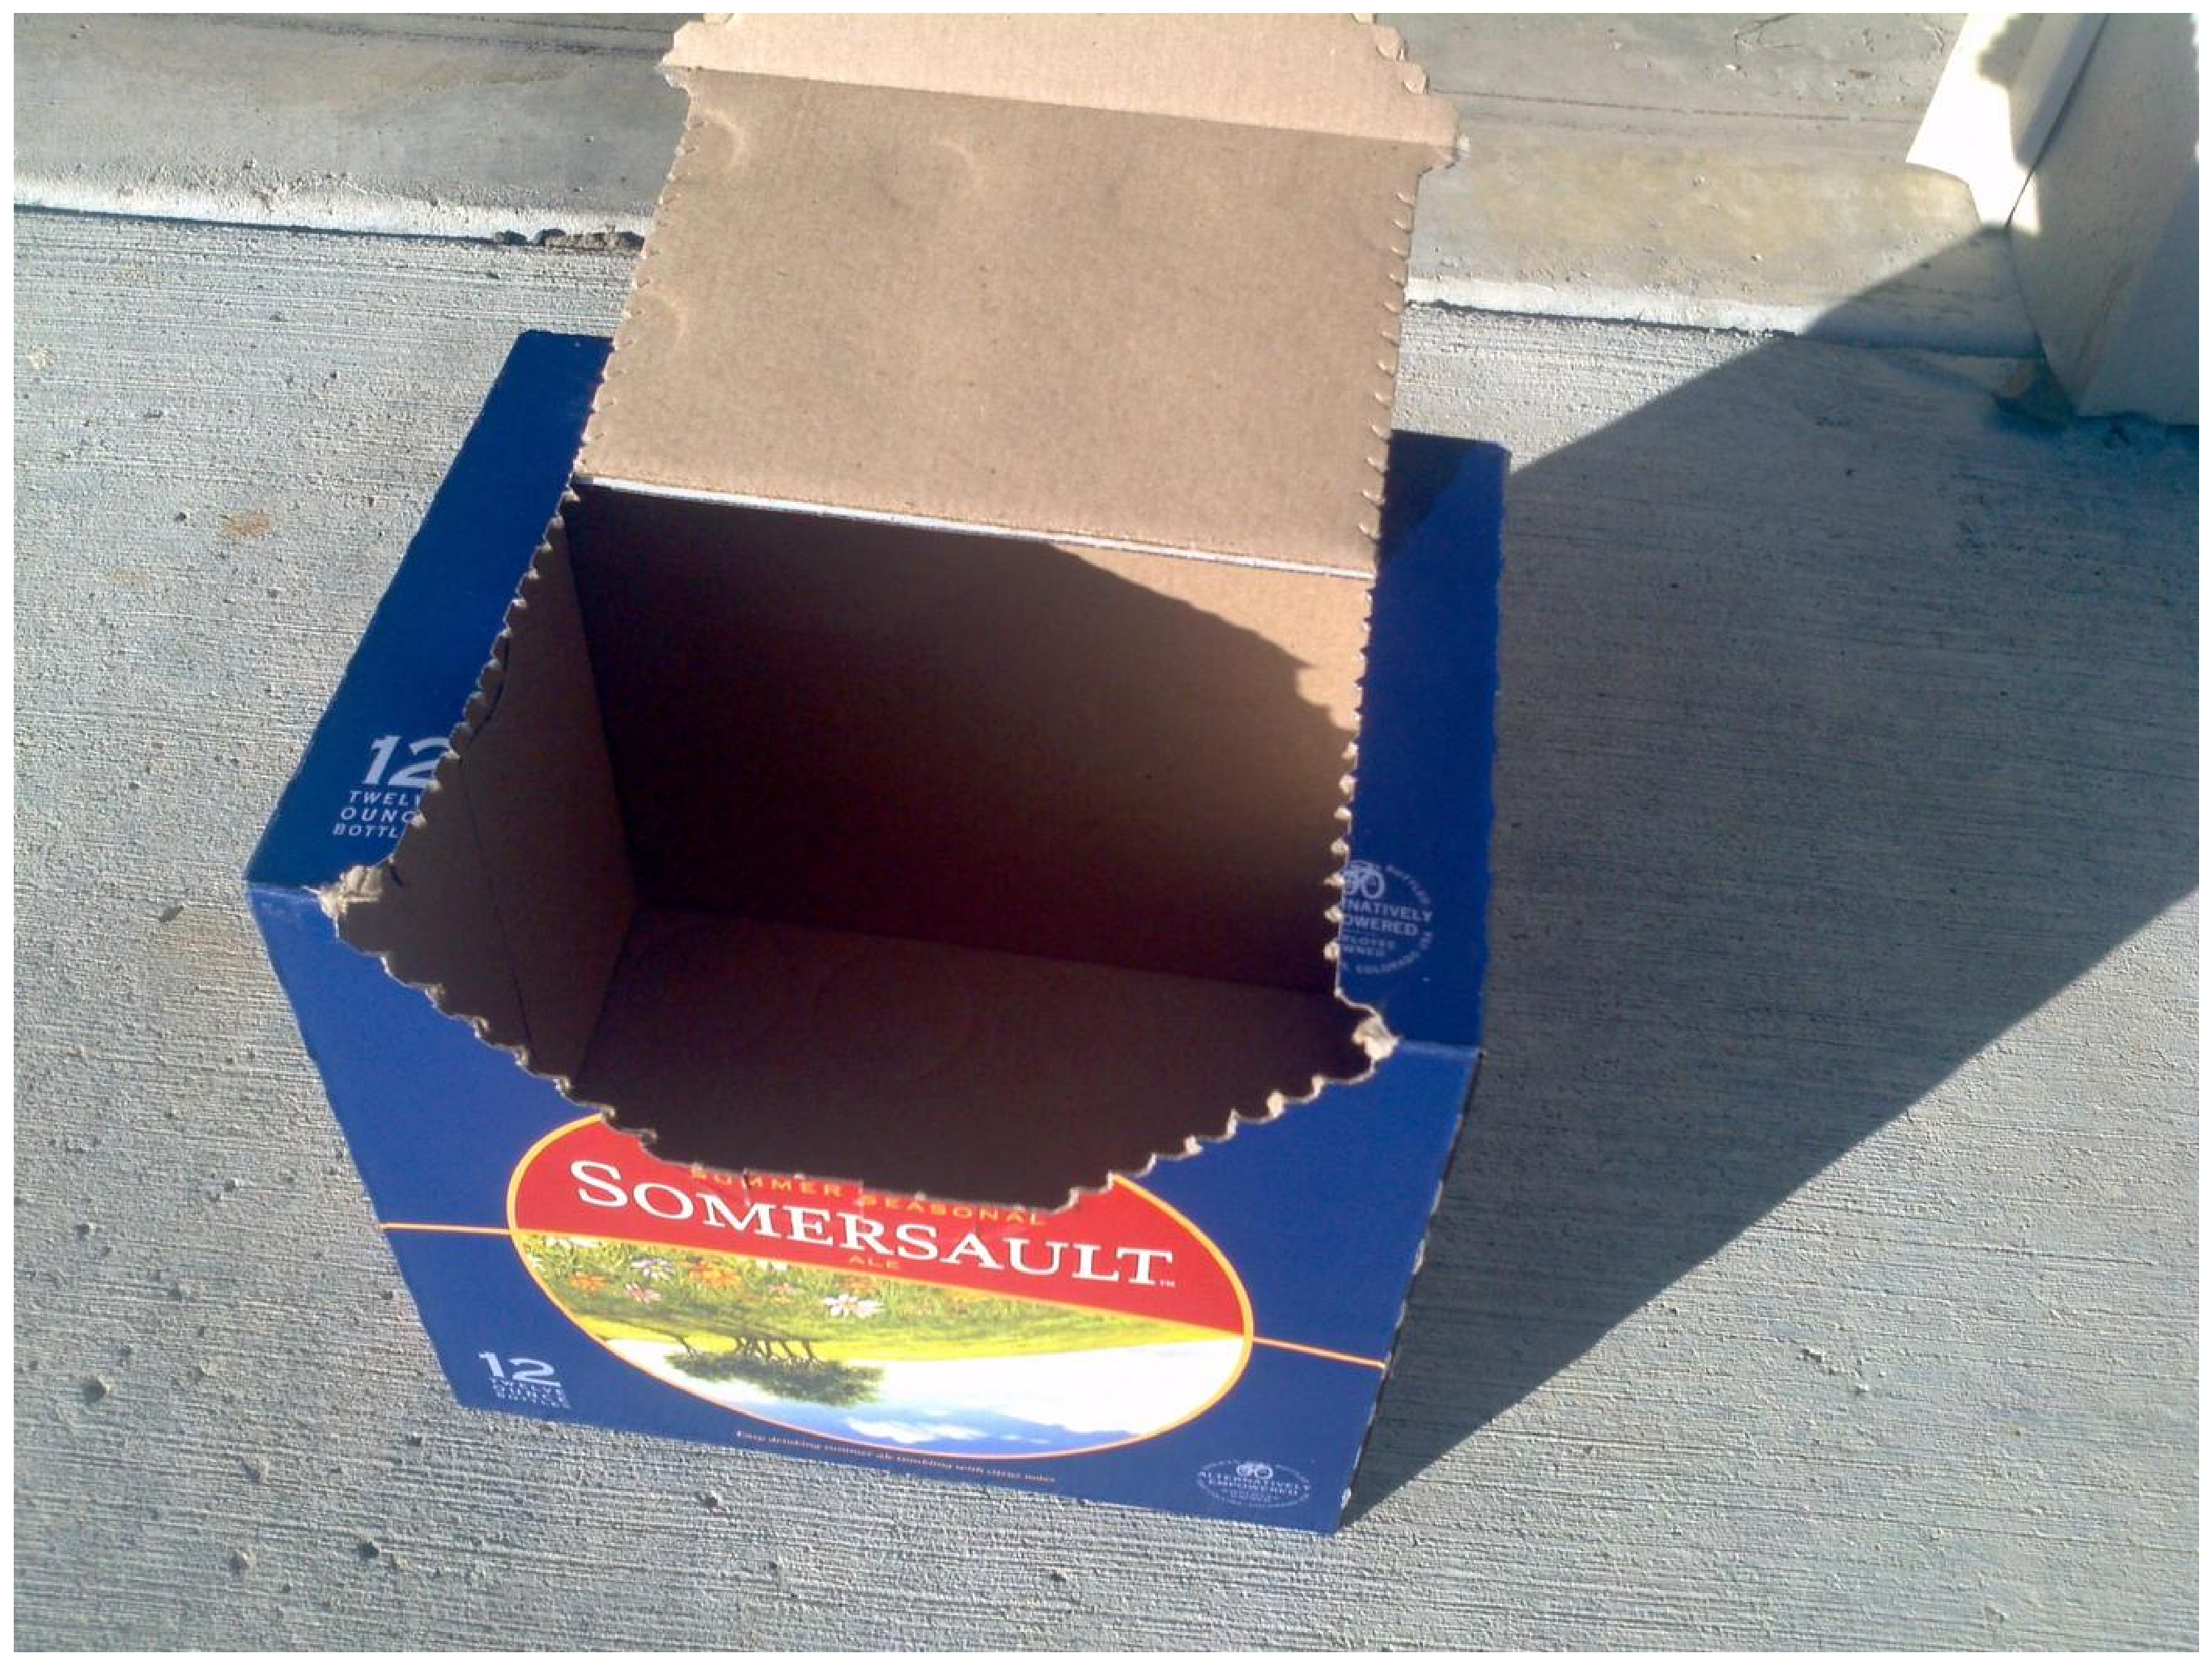
\includegraphics[width=0.8\textwidth]{eps/emptyBox.eps}
\caption{Properly 'dispose' of the contents in the box.
	 \label{fig:emptyBox}} 
\end{figure}

\begin{figure}[ht!]
\centering
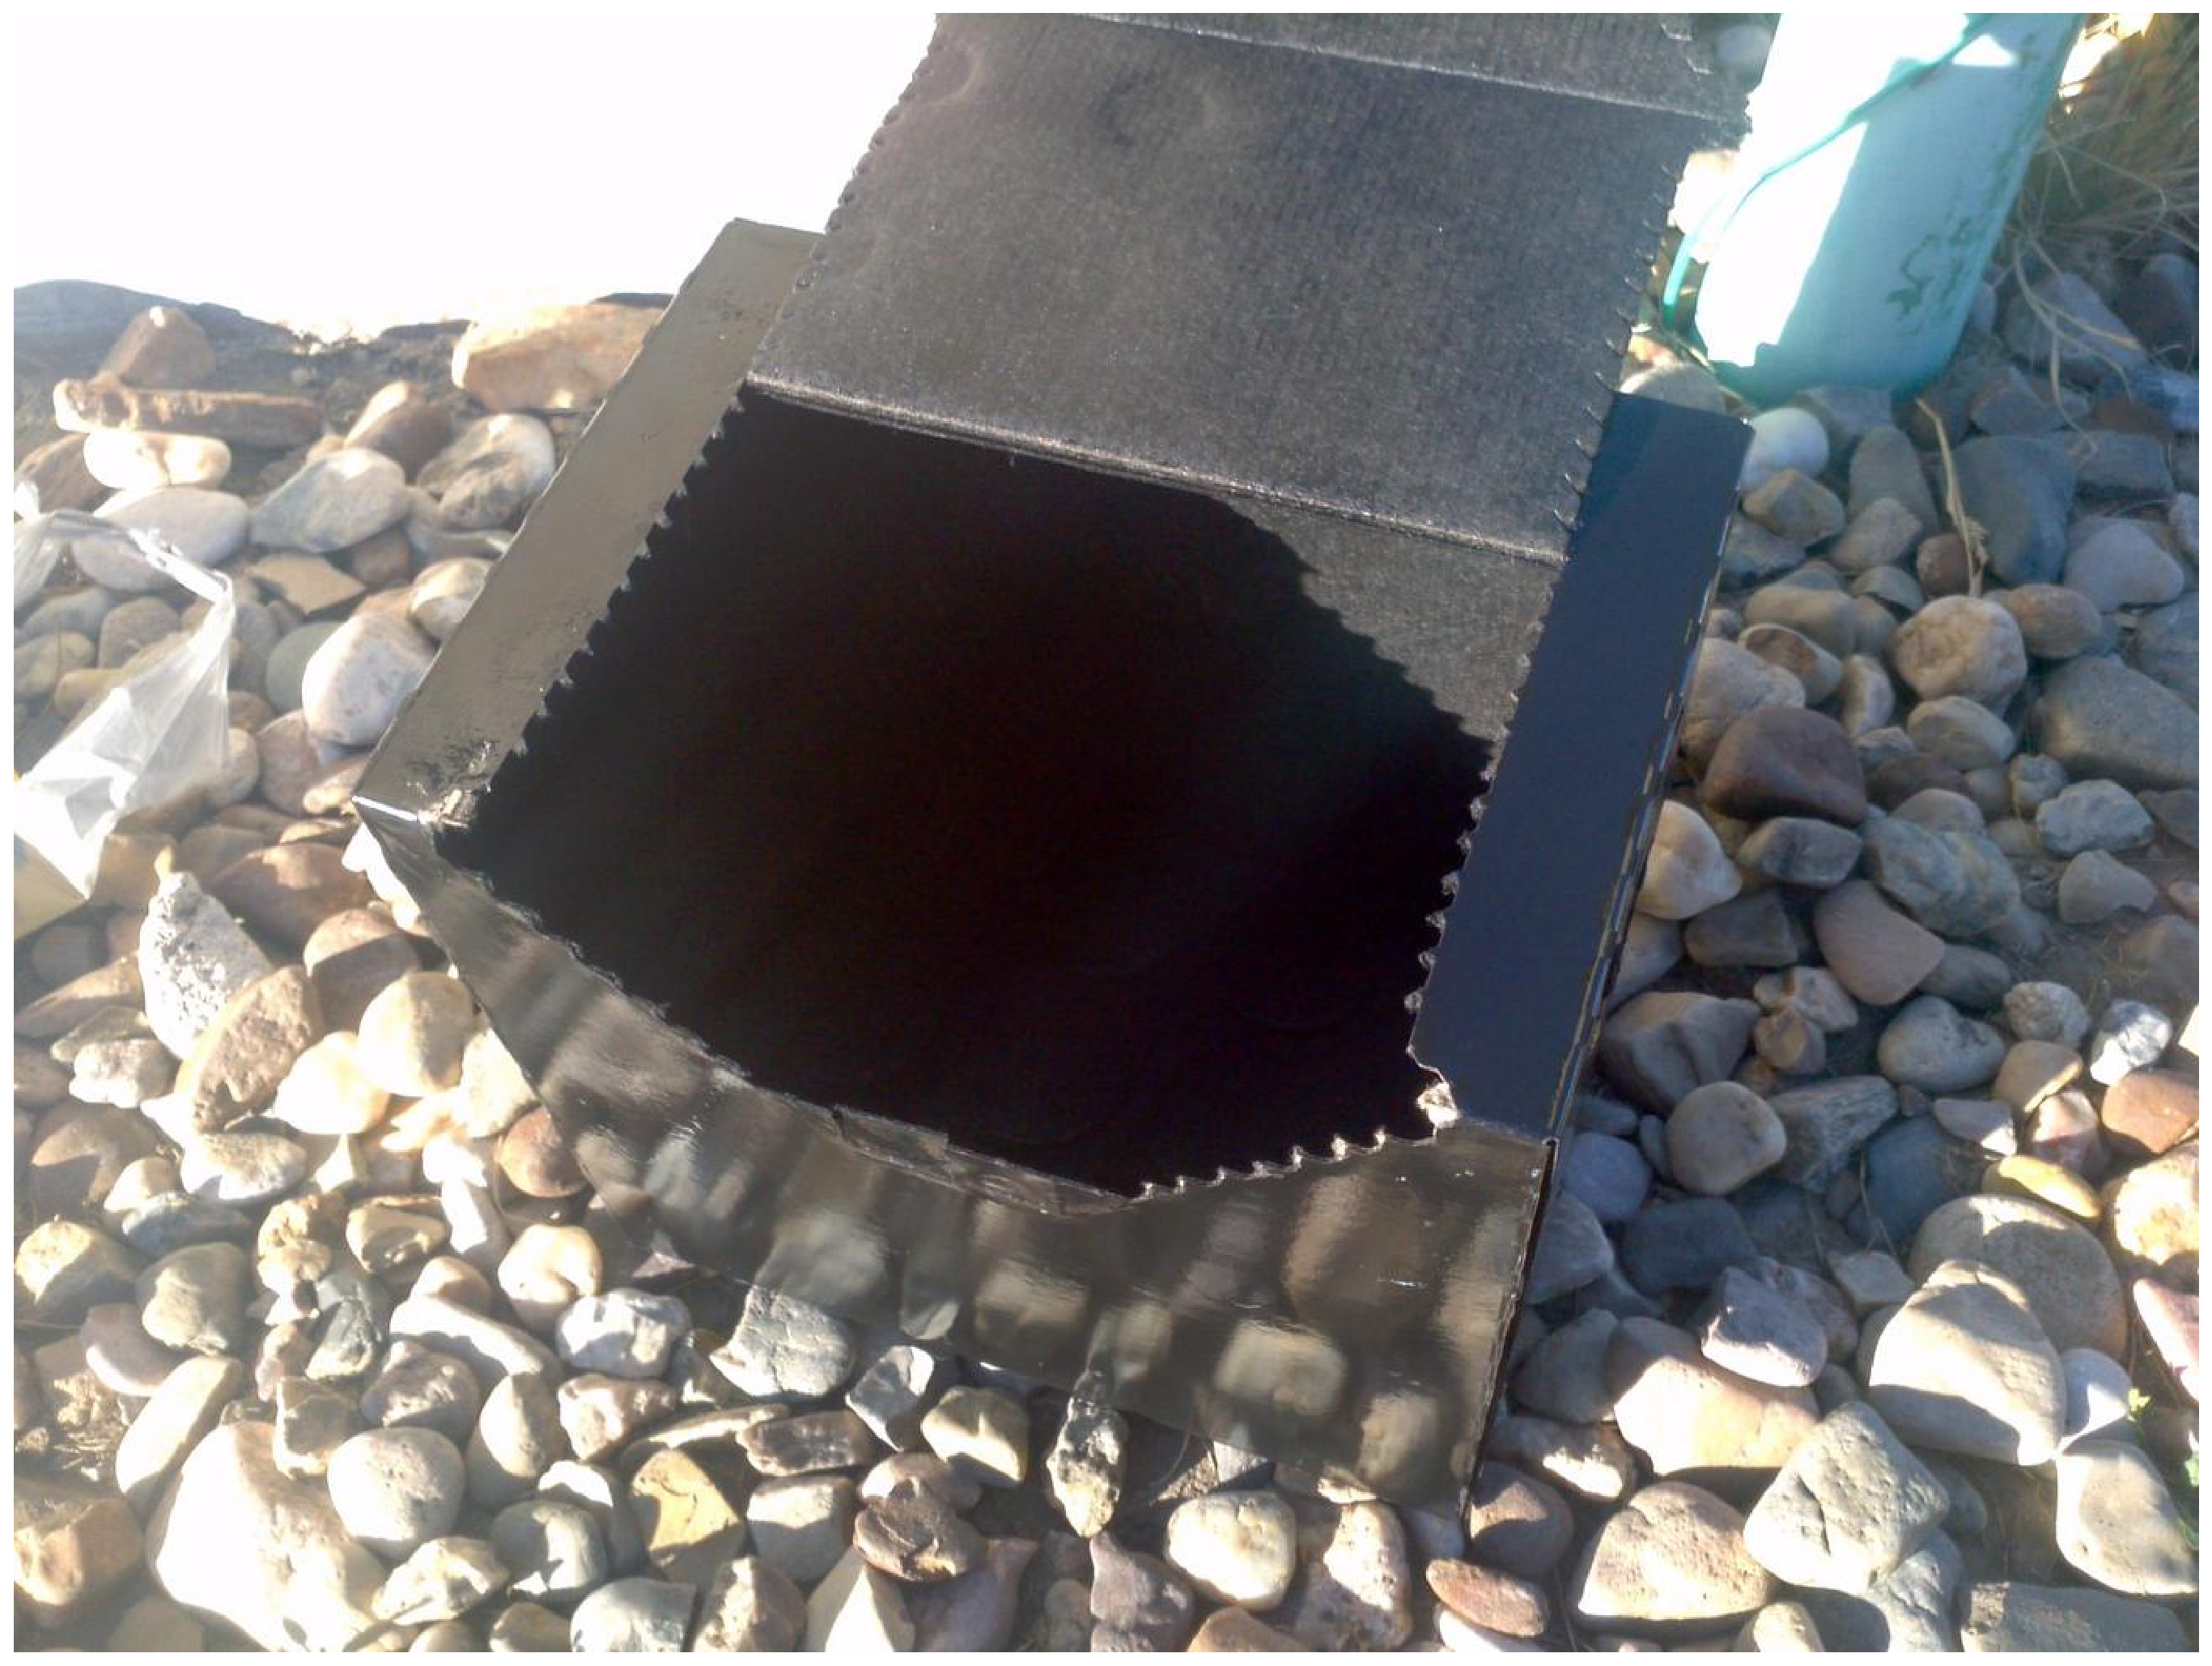
\includegraphics[width=0.8\textwidth]{eps/blackBox.eps}
\caption{Use black spray paint to make the box black on the inside and outside so that it absorbs light where it should be.
	 \label{fig:blackBox}} 
\end{figure}

\begin{figure}[ht!]
\centering
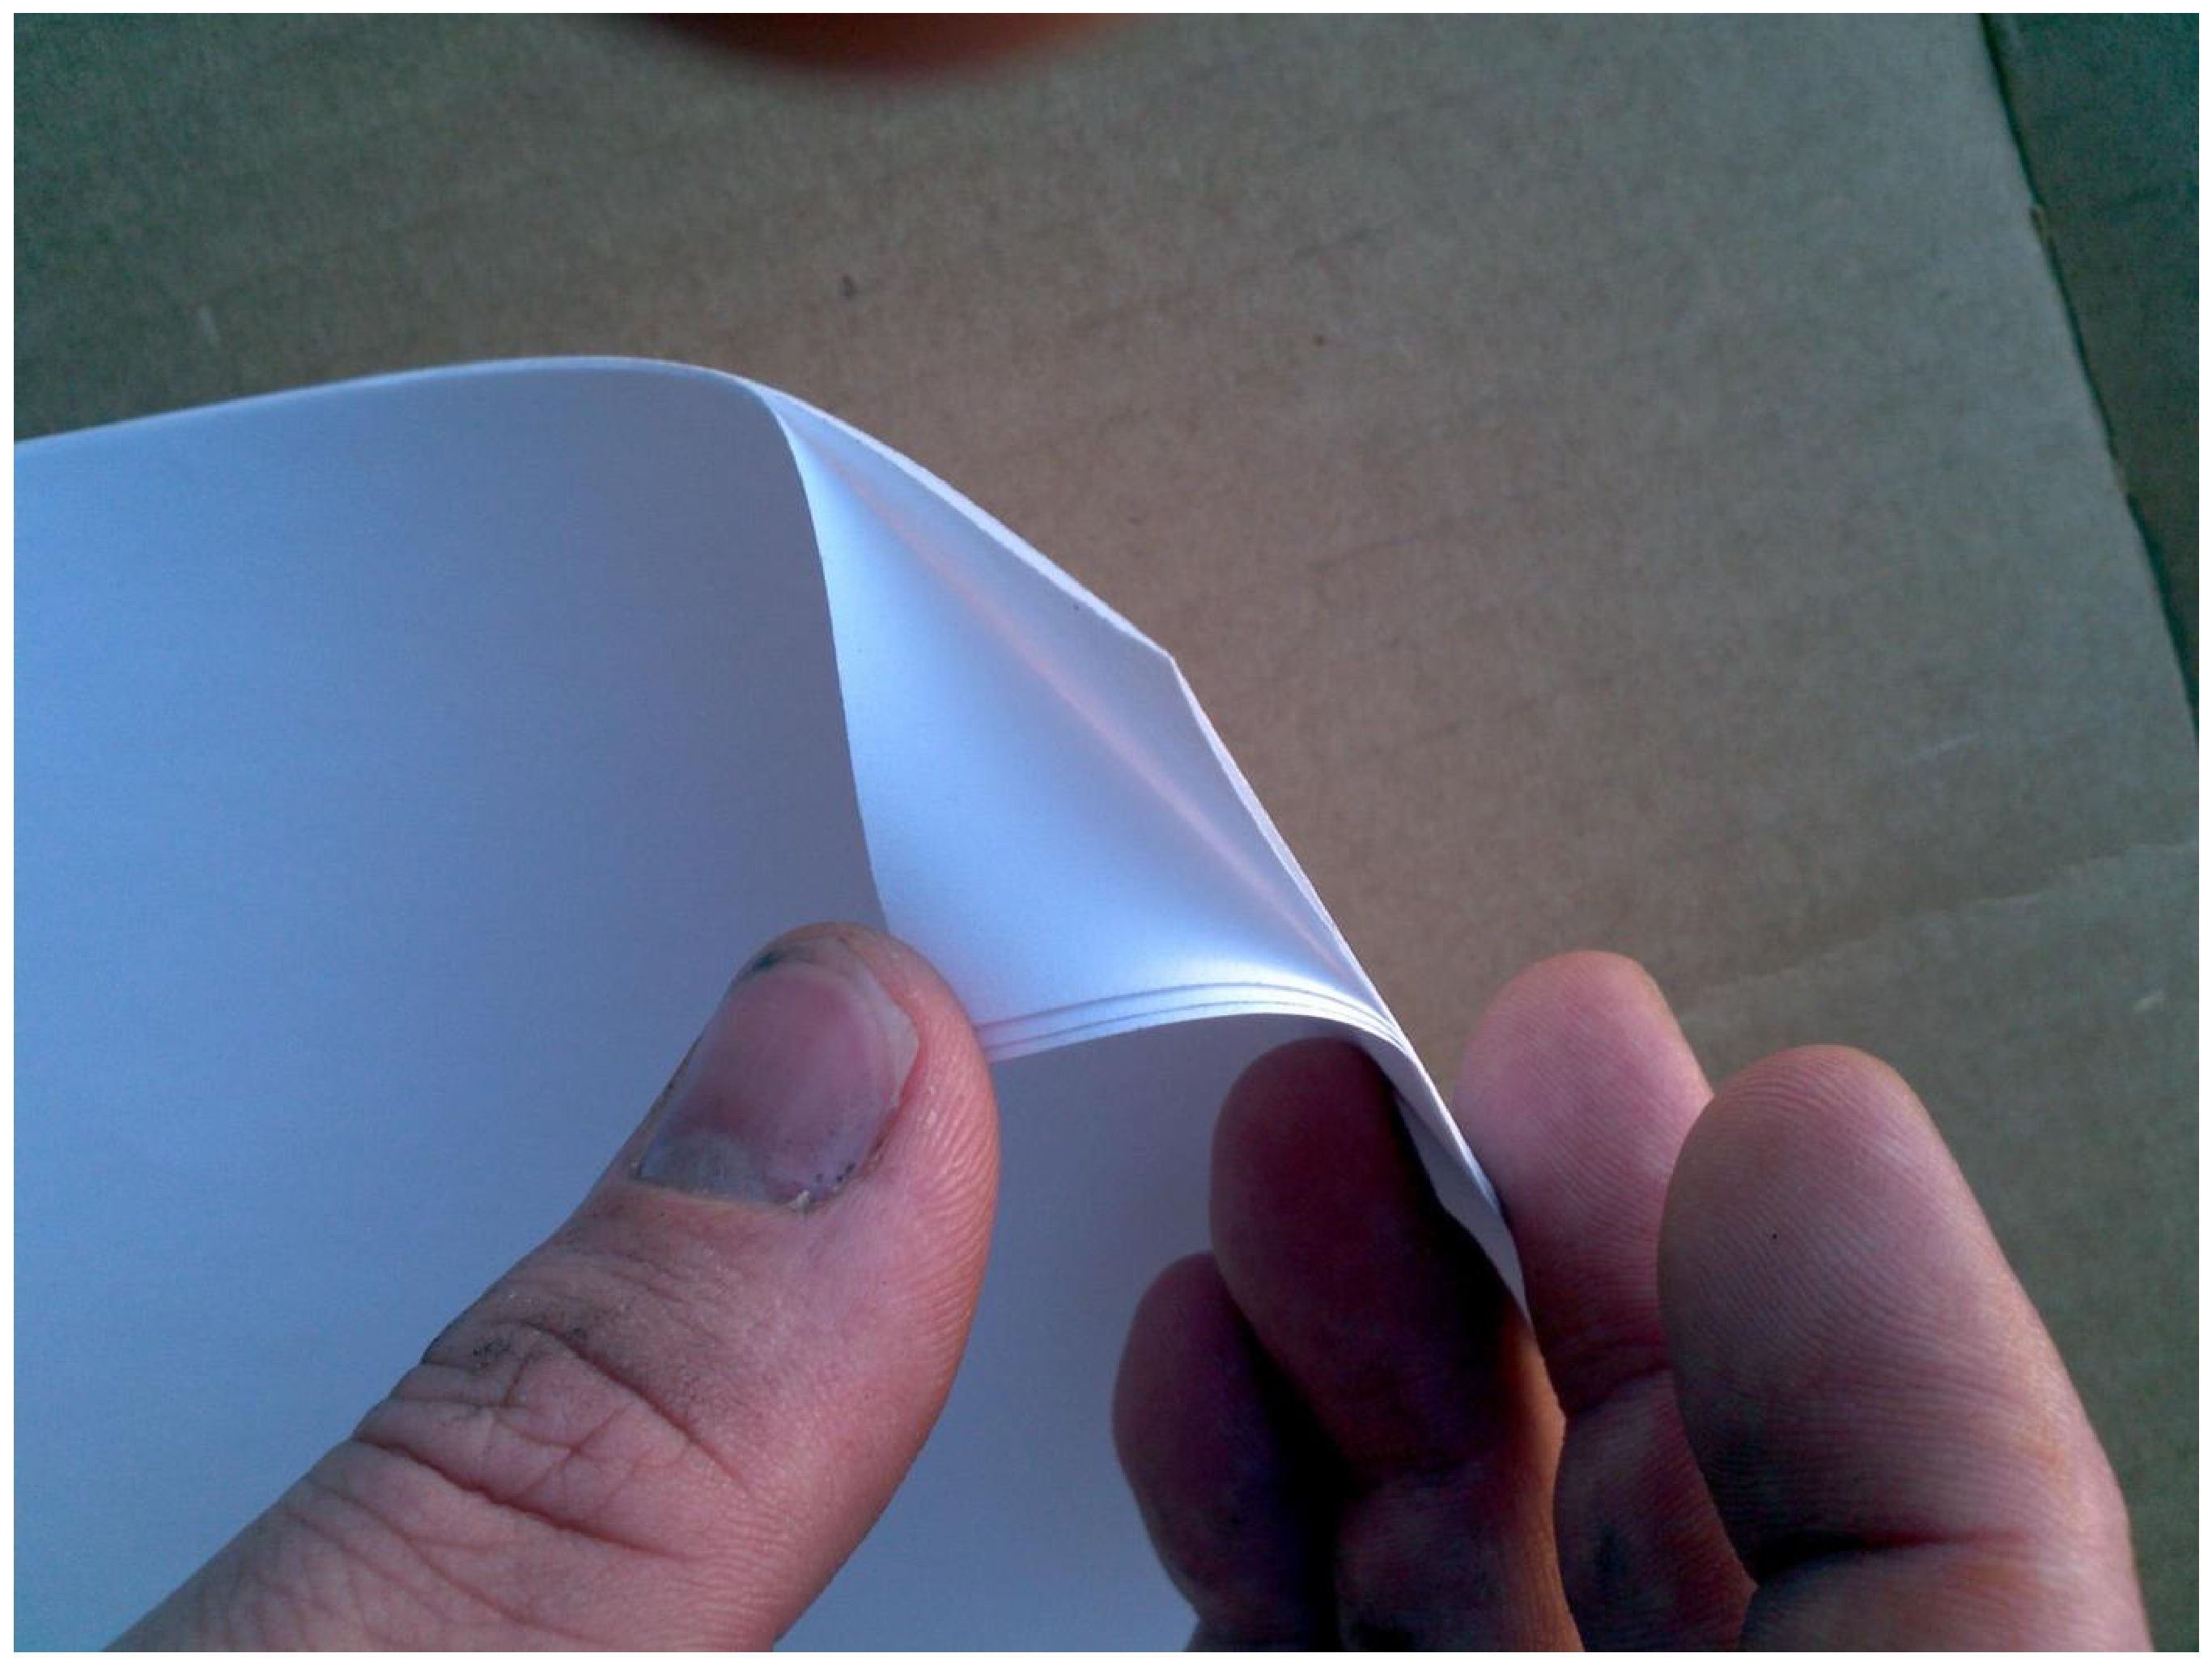
\includegraphics[width=0.8\textwidth]{eps/paperLayer.eps}
\caption{Measure one wall of the box and cut out white paper pieces to fit those dimensions.}
\end{figure}

\begin{figure}[ht!]
\centering
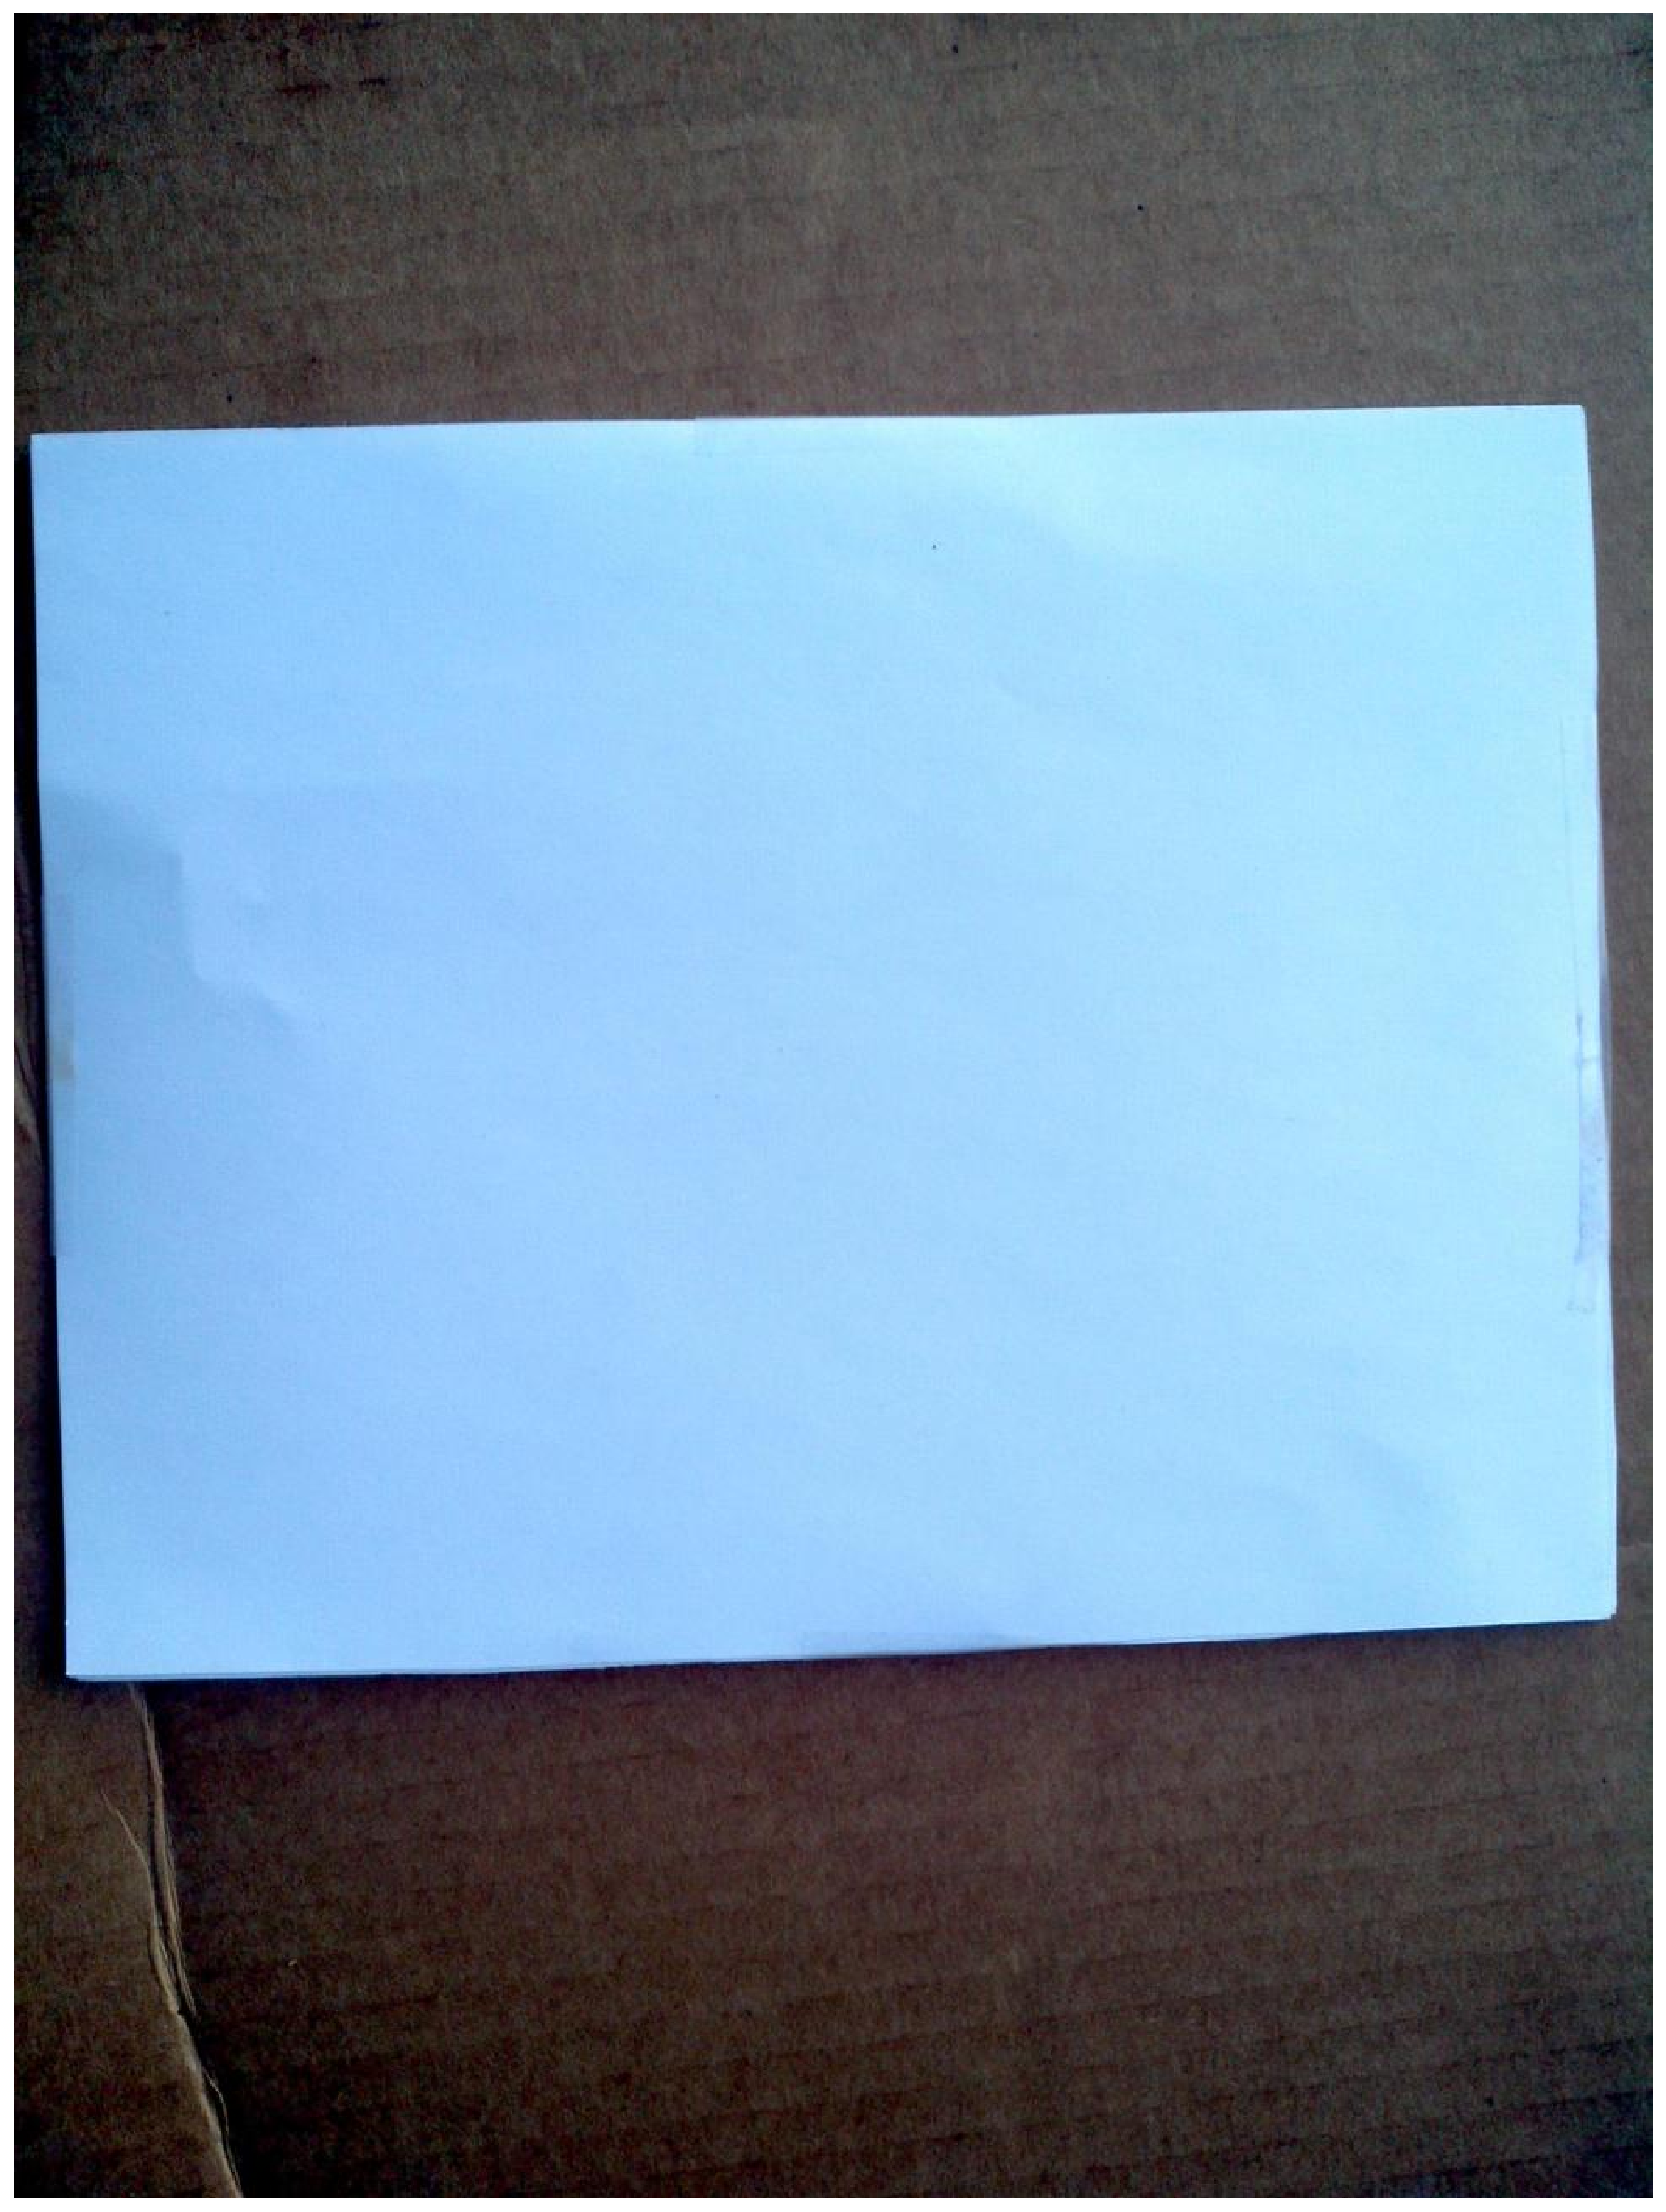
\includegraphics[width=0.8\textwidth]{eps/layersAligned.eps}
\caption{Stack the paper pieces on top of each other and line them up. Layers are used here to reduce light emission through the paper and increase reflectance.}
\end{figure}

\begin{figure}[ht!]
\centering
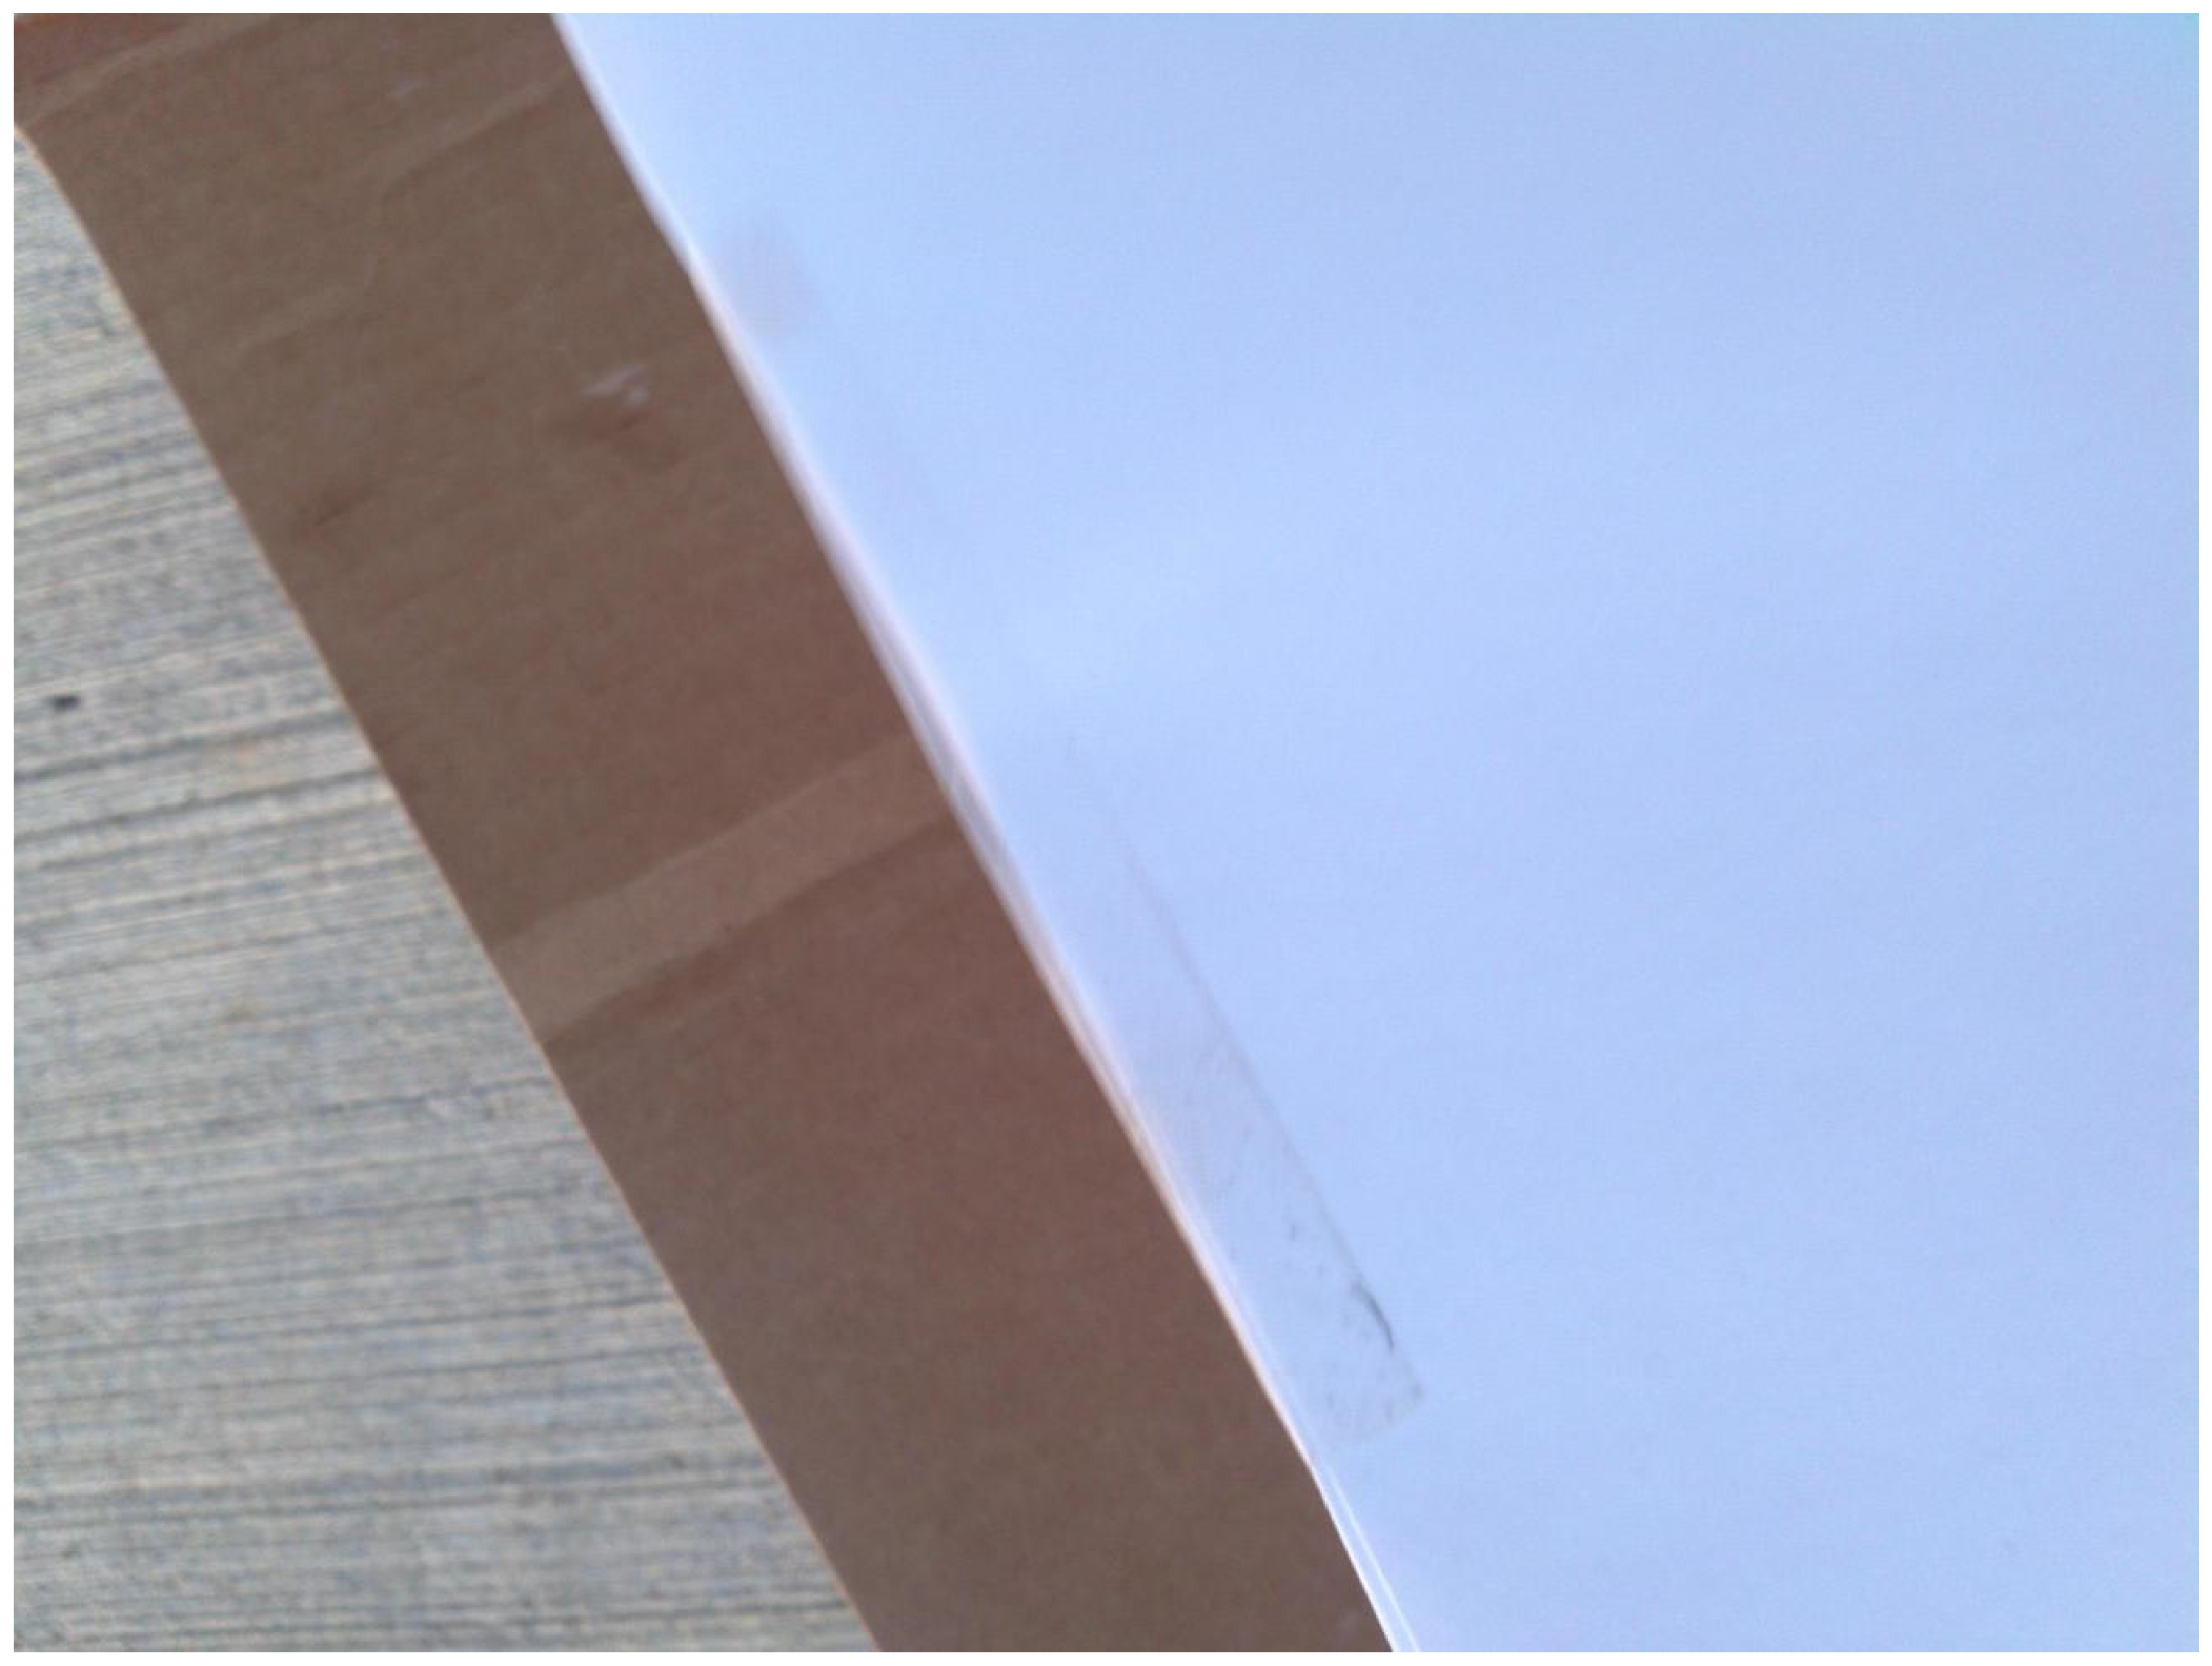
\includegraphics[width=0.8\textwidth]{eps/layersTaped.eps}
\caption{Use a minimal amount of scotch tape to tape the edges of the papers together so that they stay together.}
\end{figure}

\begin{figure}[ht!]
\centering
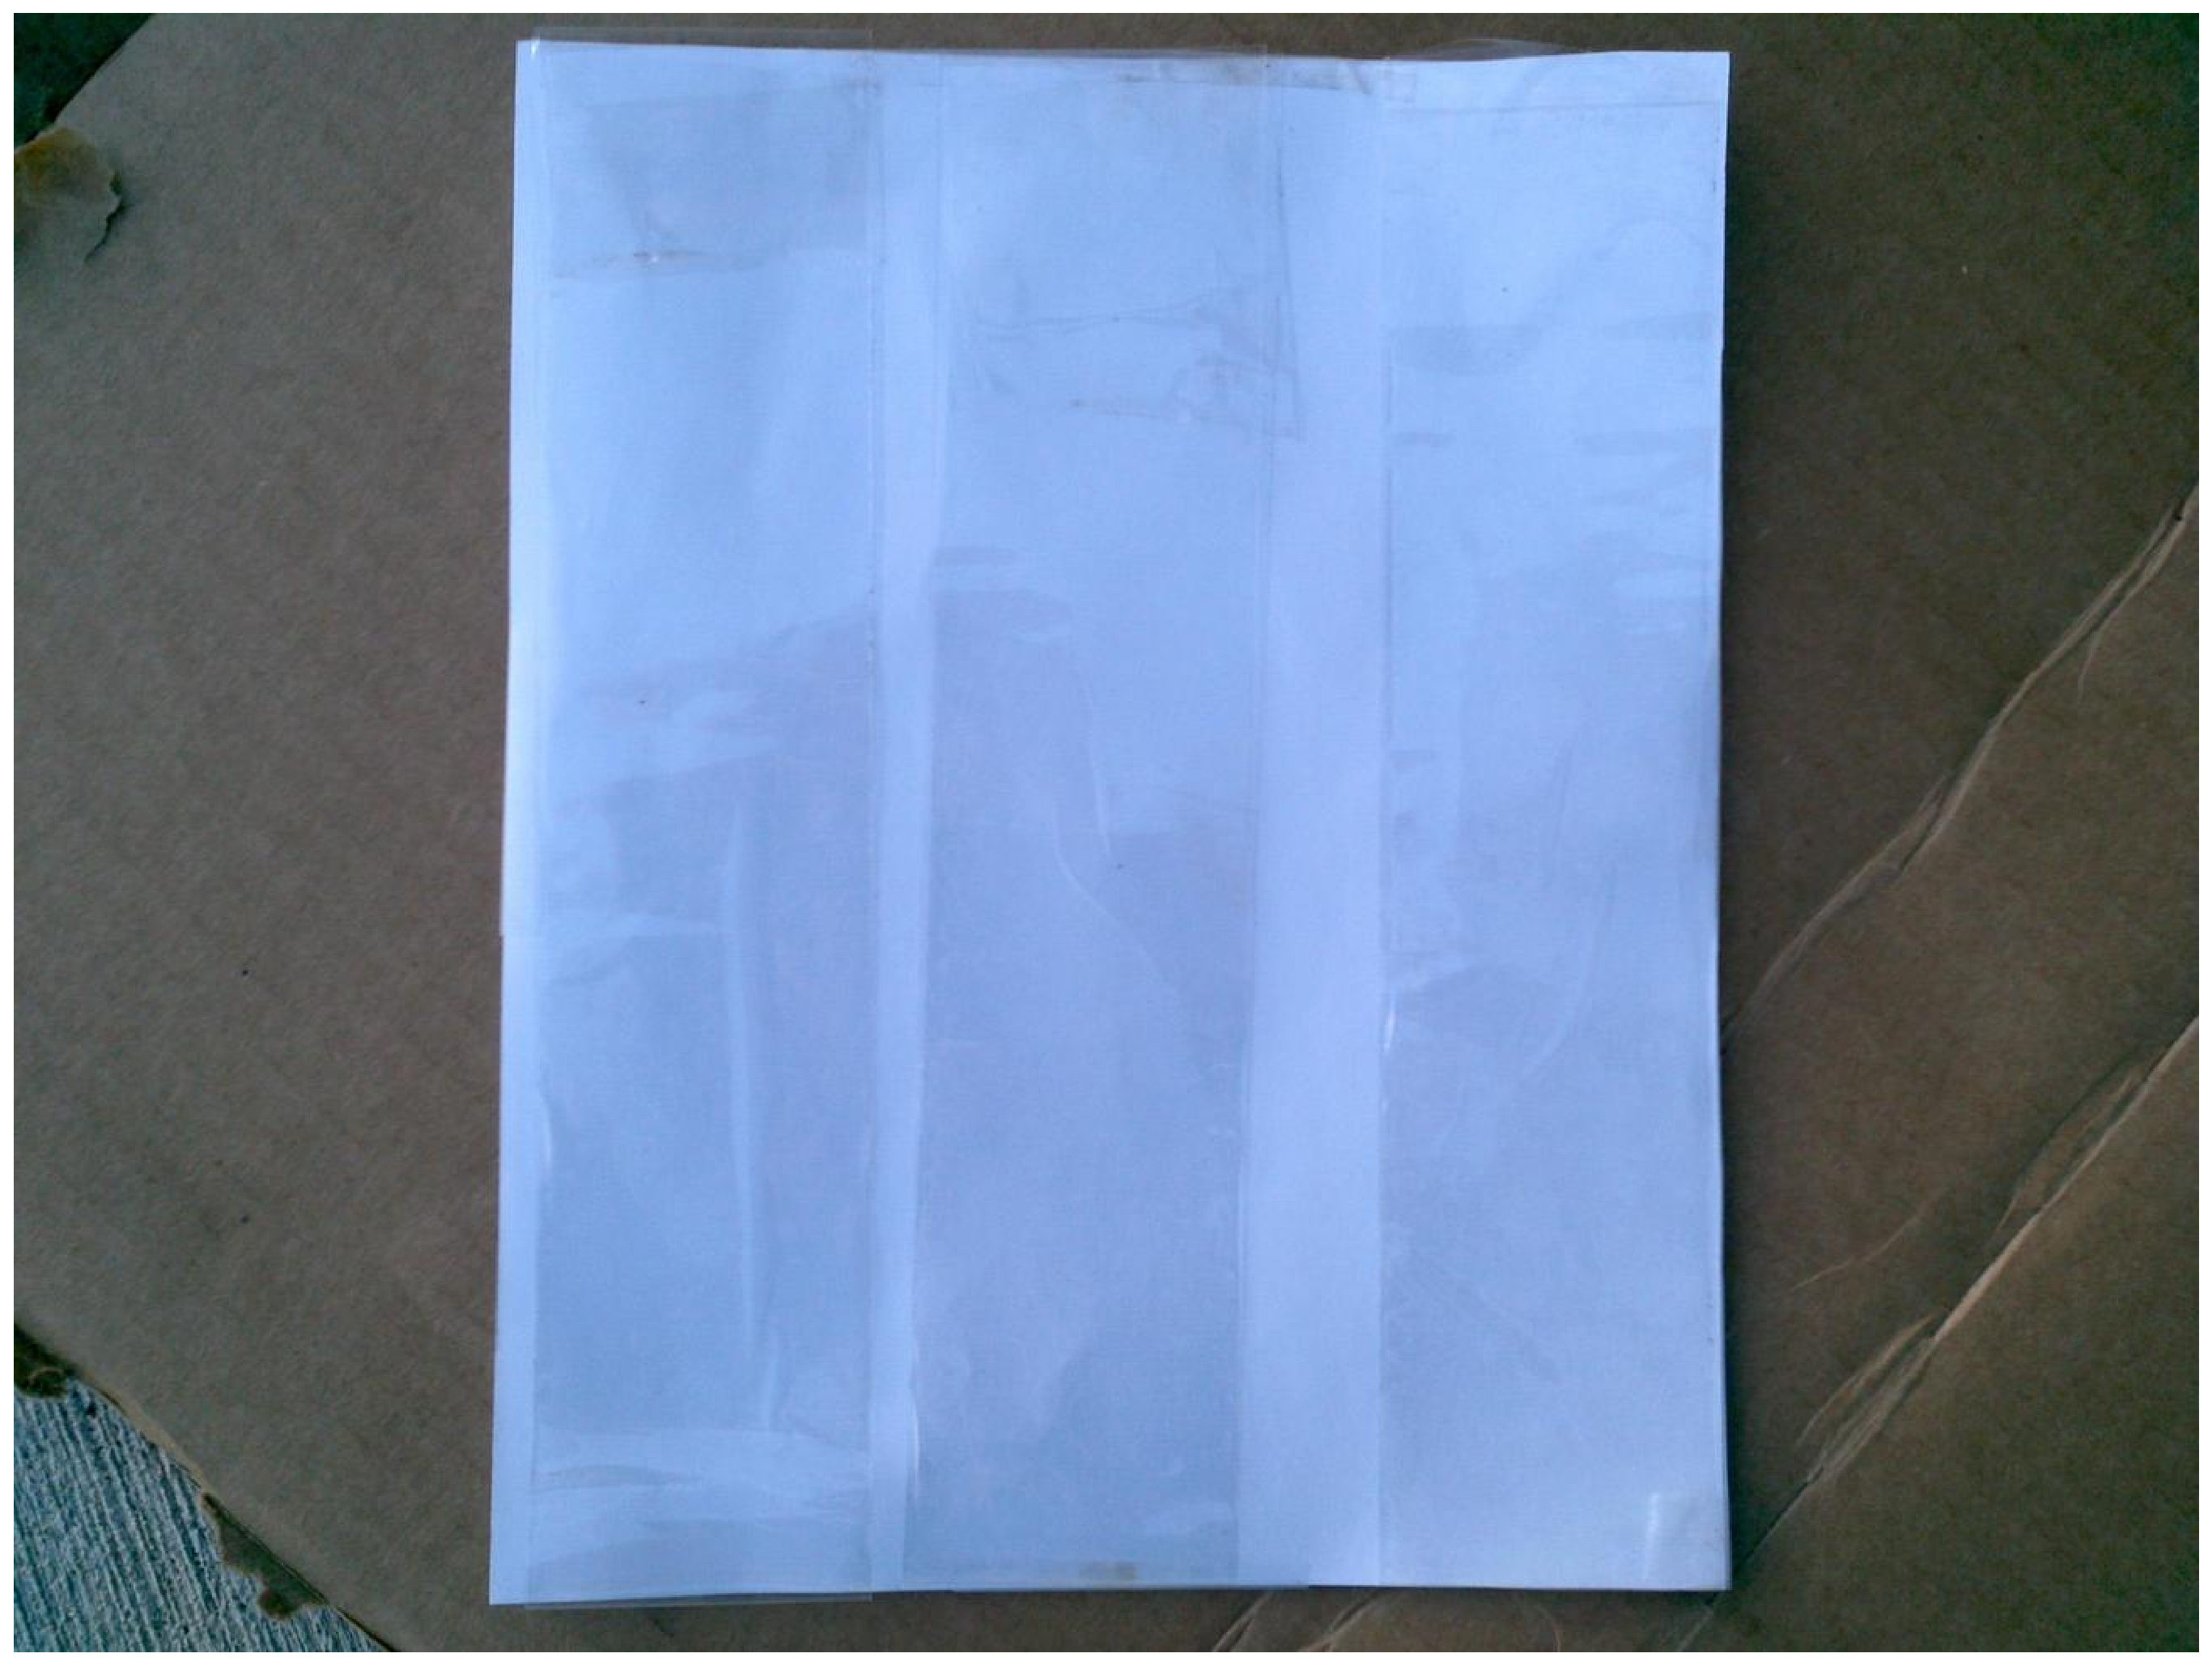
\includegraphics[width=0.8\textwidth]{eps/doubleSided.eps}
\caption{Place some strips of double sided tape across one side of the paper stack.}
\end{figure}

\begin{figure}[ht!]
\centering
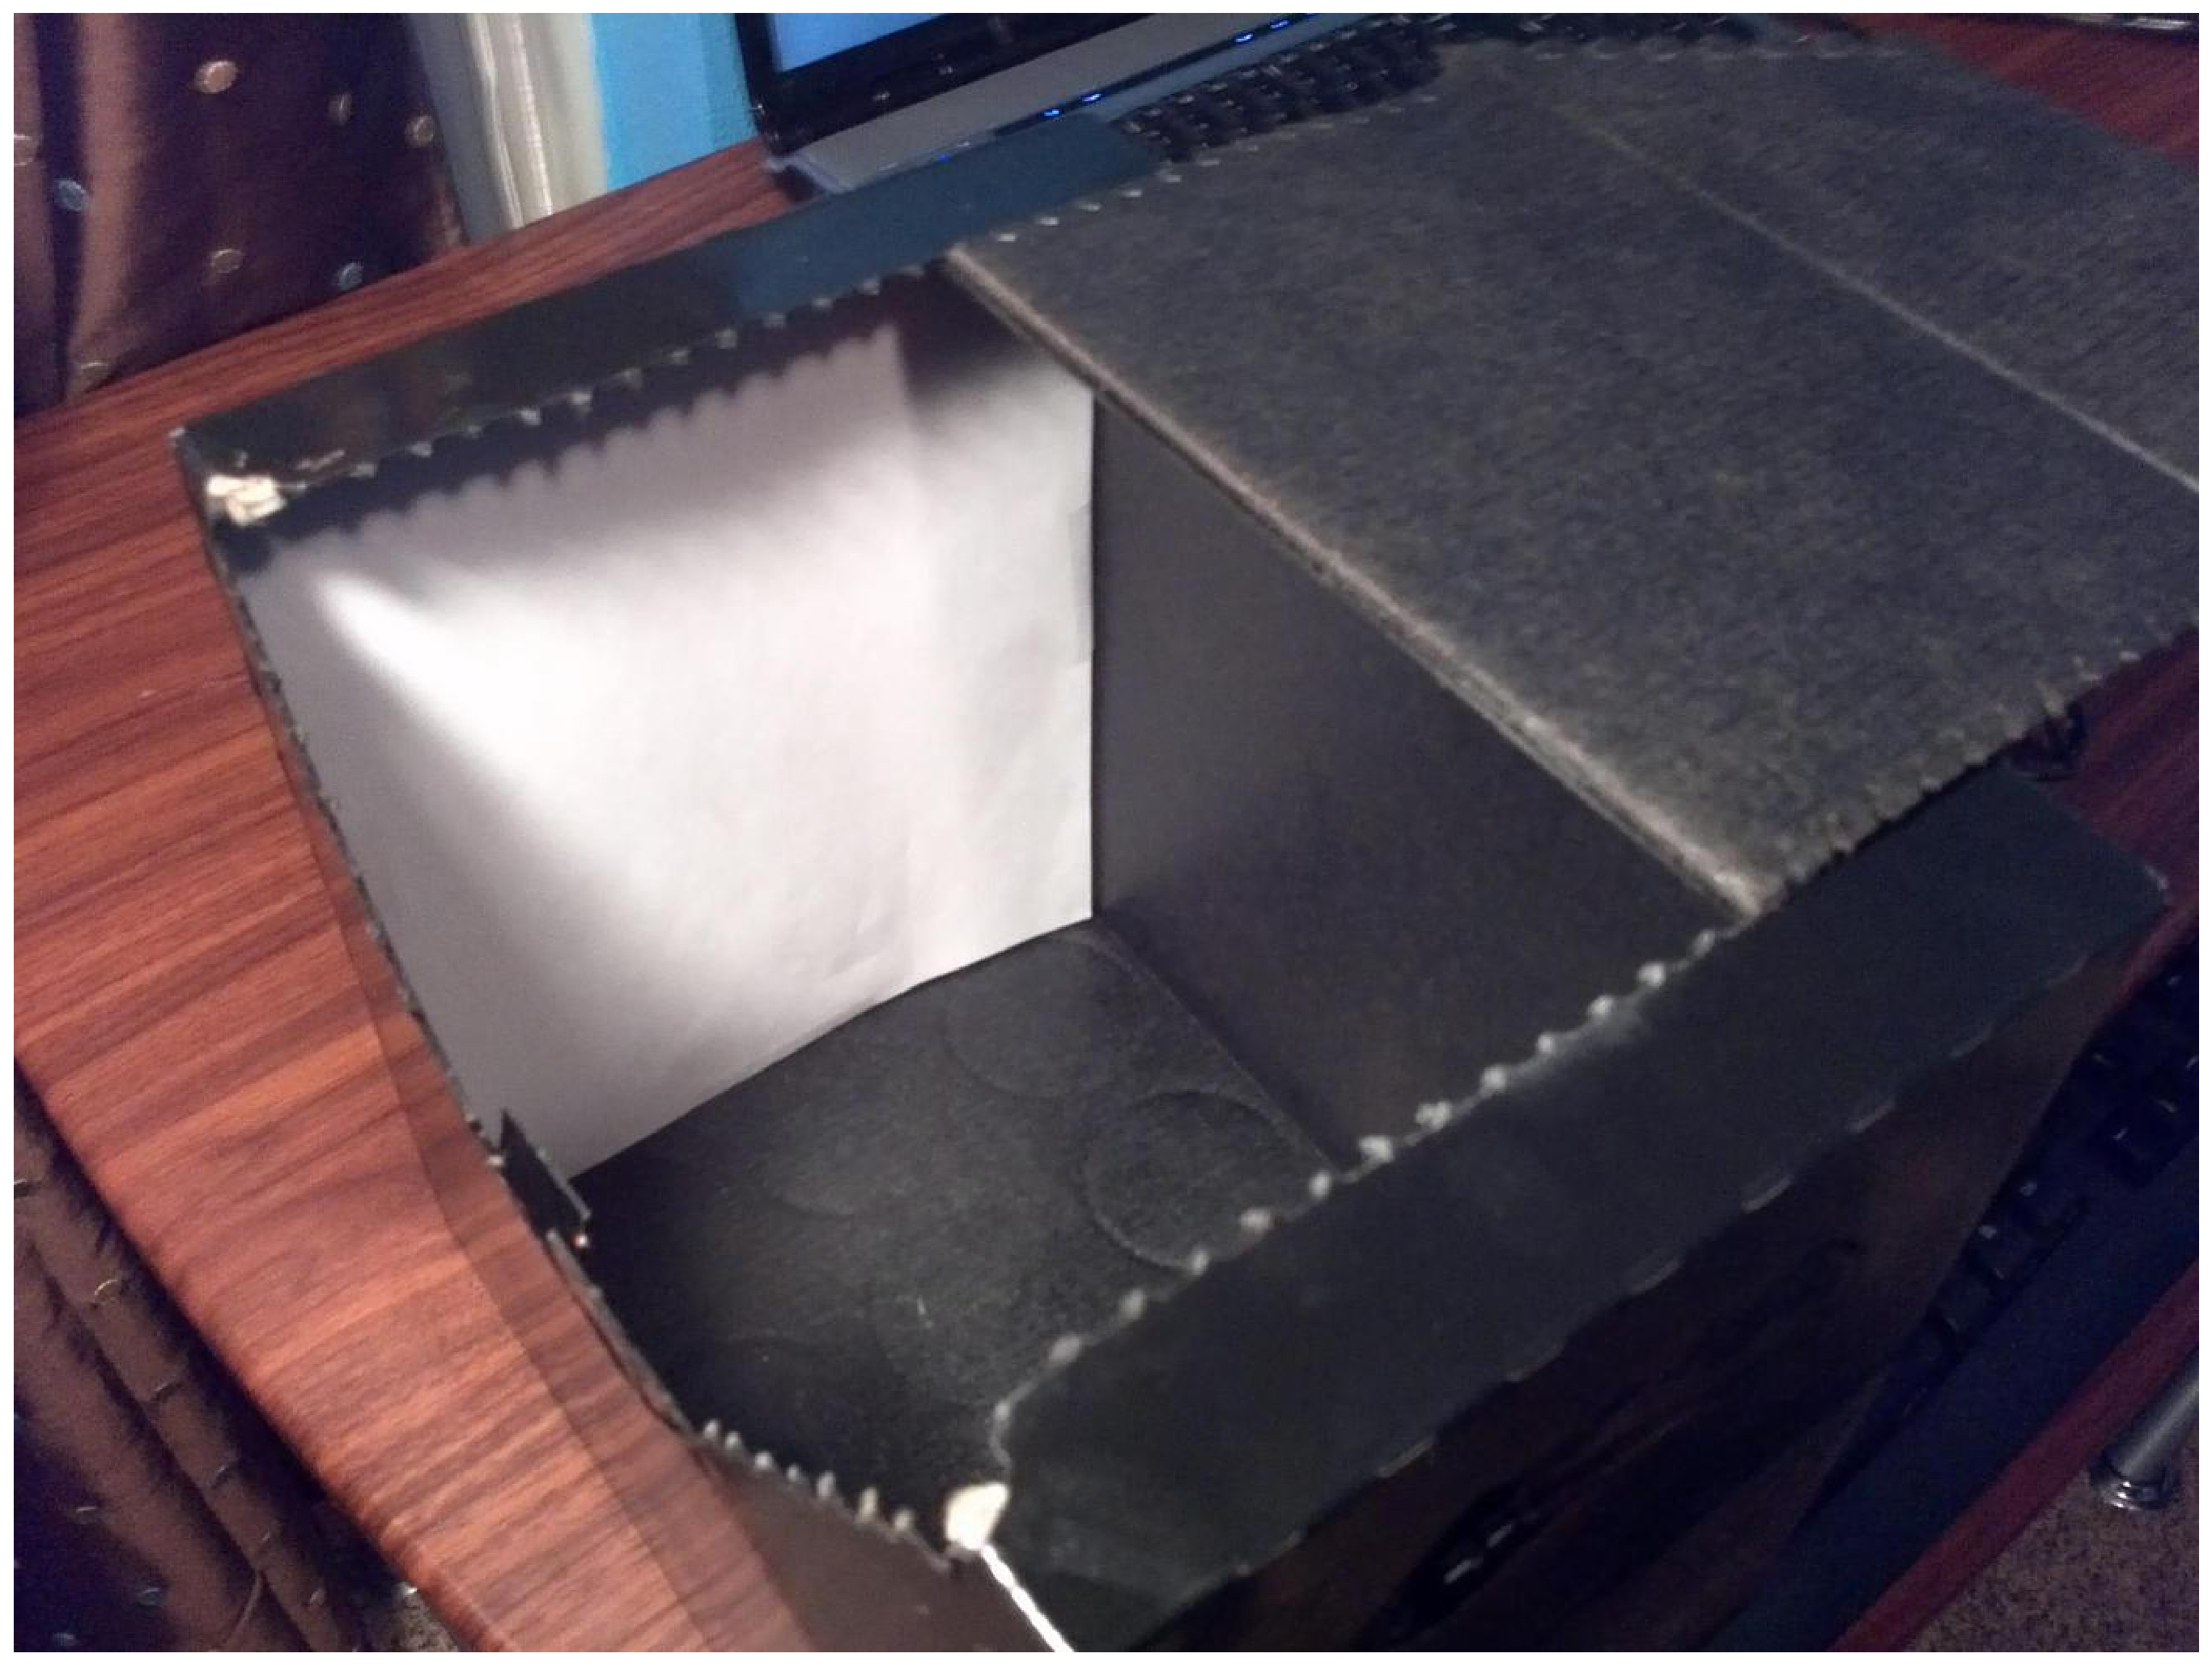
\includegraphics[width=0.8\textwidth]{eps/tapedIn.eps}
\caption{Adhere the paper stack to one of the inner walls of the box that matches the dimensions that the paper stack was cut to.}
\end{figure}

\begin{figure}[ht!]
\centering
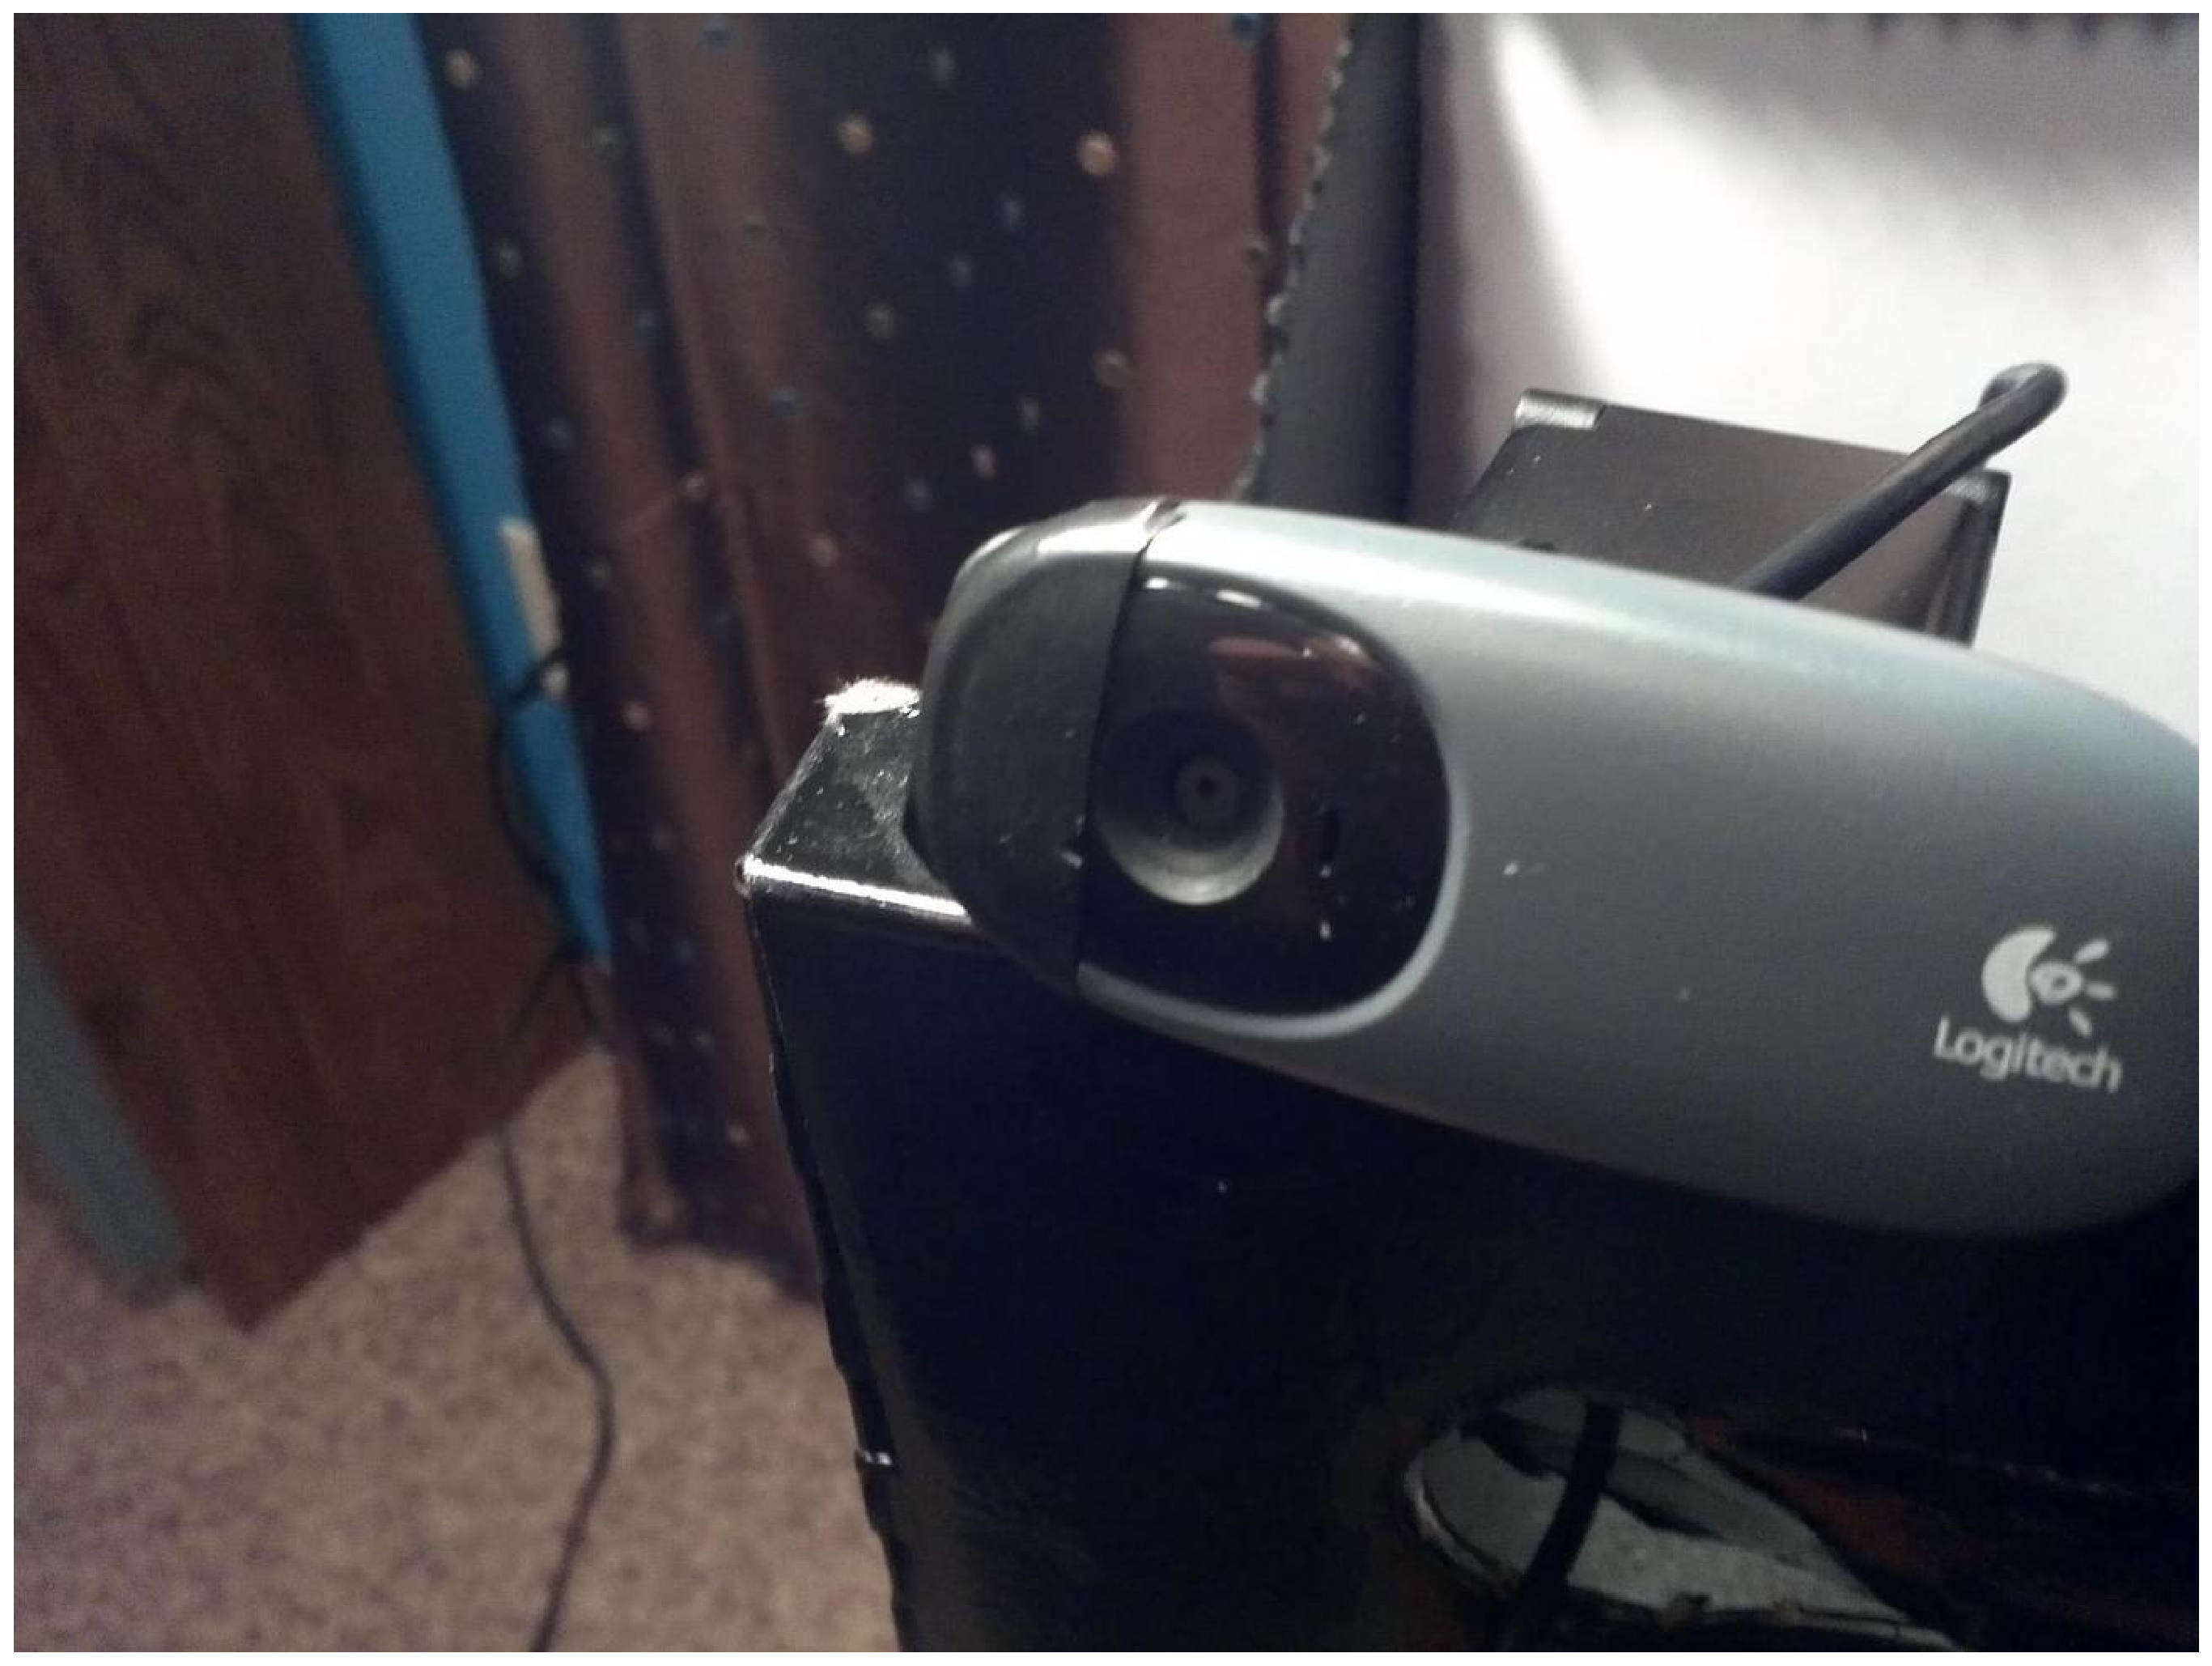
\includegraphics[width=0.8\textwidth]{eps/webCam.eps}
\caption{Find a webcam that will fit nicely inside of the box. If your webcam has a power light make sure to put a piece of tape over it as seen in the picture.}
\end{figure}

\begin{figure}[ht!]
\centering
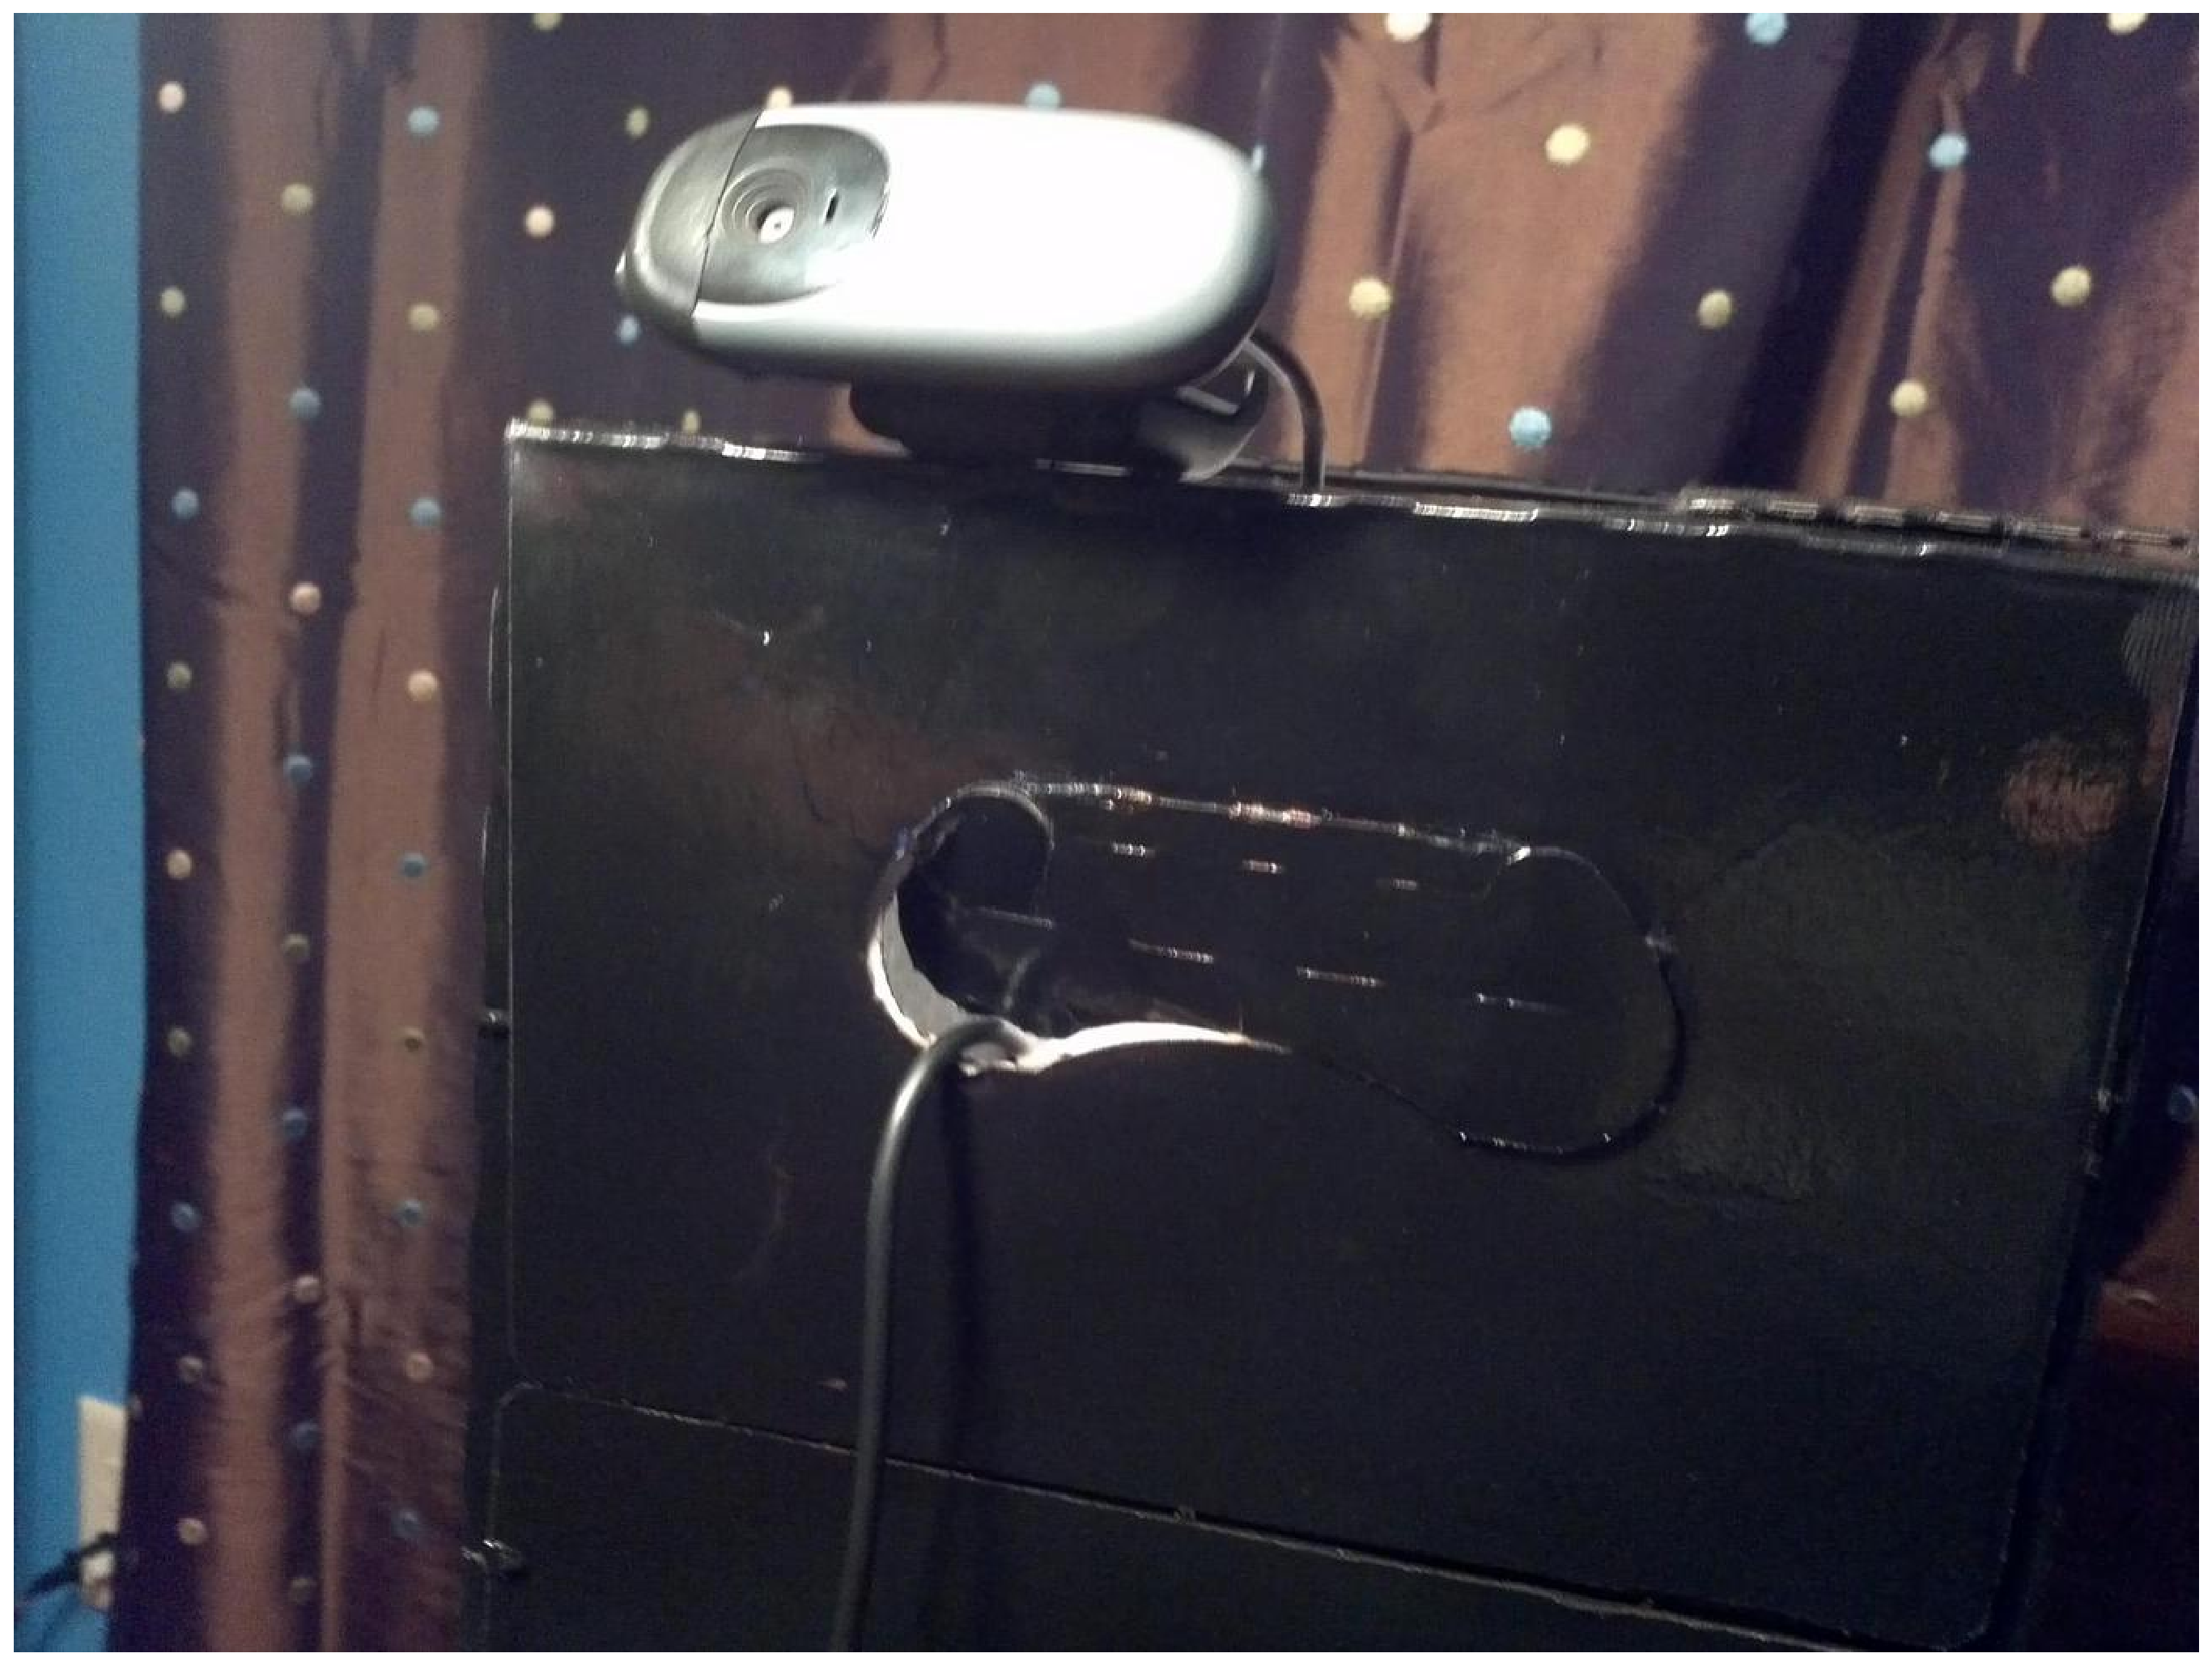
\includegraphics[width=0.8\textwidth]{eps/webcamCord.eps}
\caption{If the box already has a hole then run the webcam cord through that as shown. Otherwise make a suitable hole.}
\end{figure}

\begin{figure}[ht!]
\centering
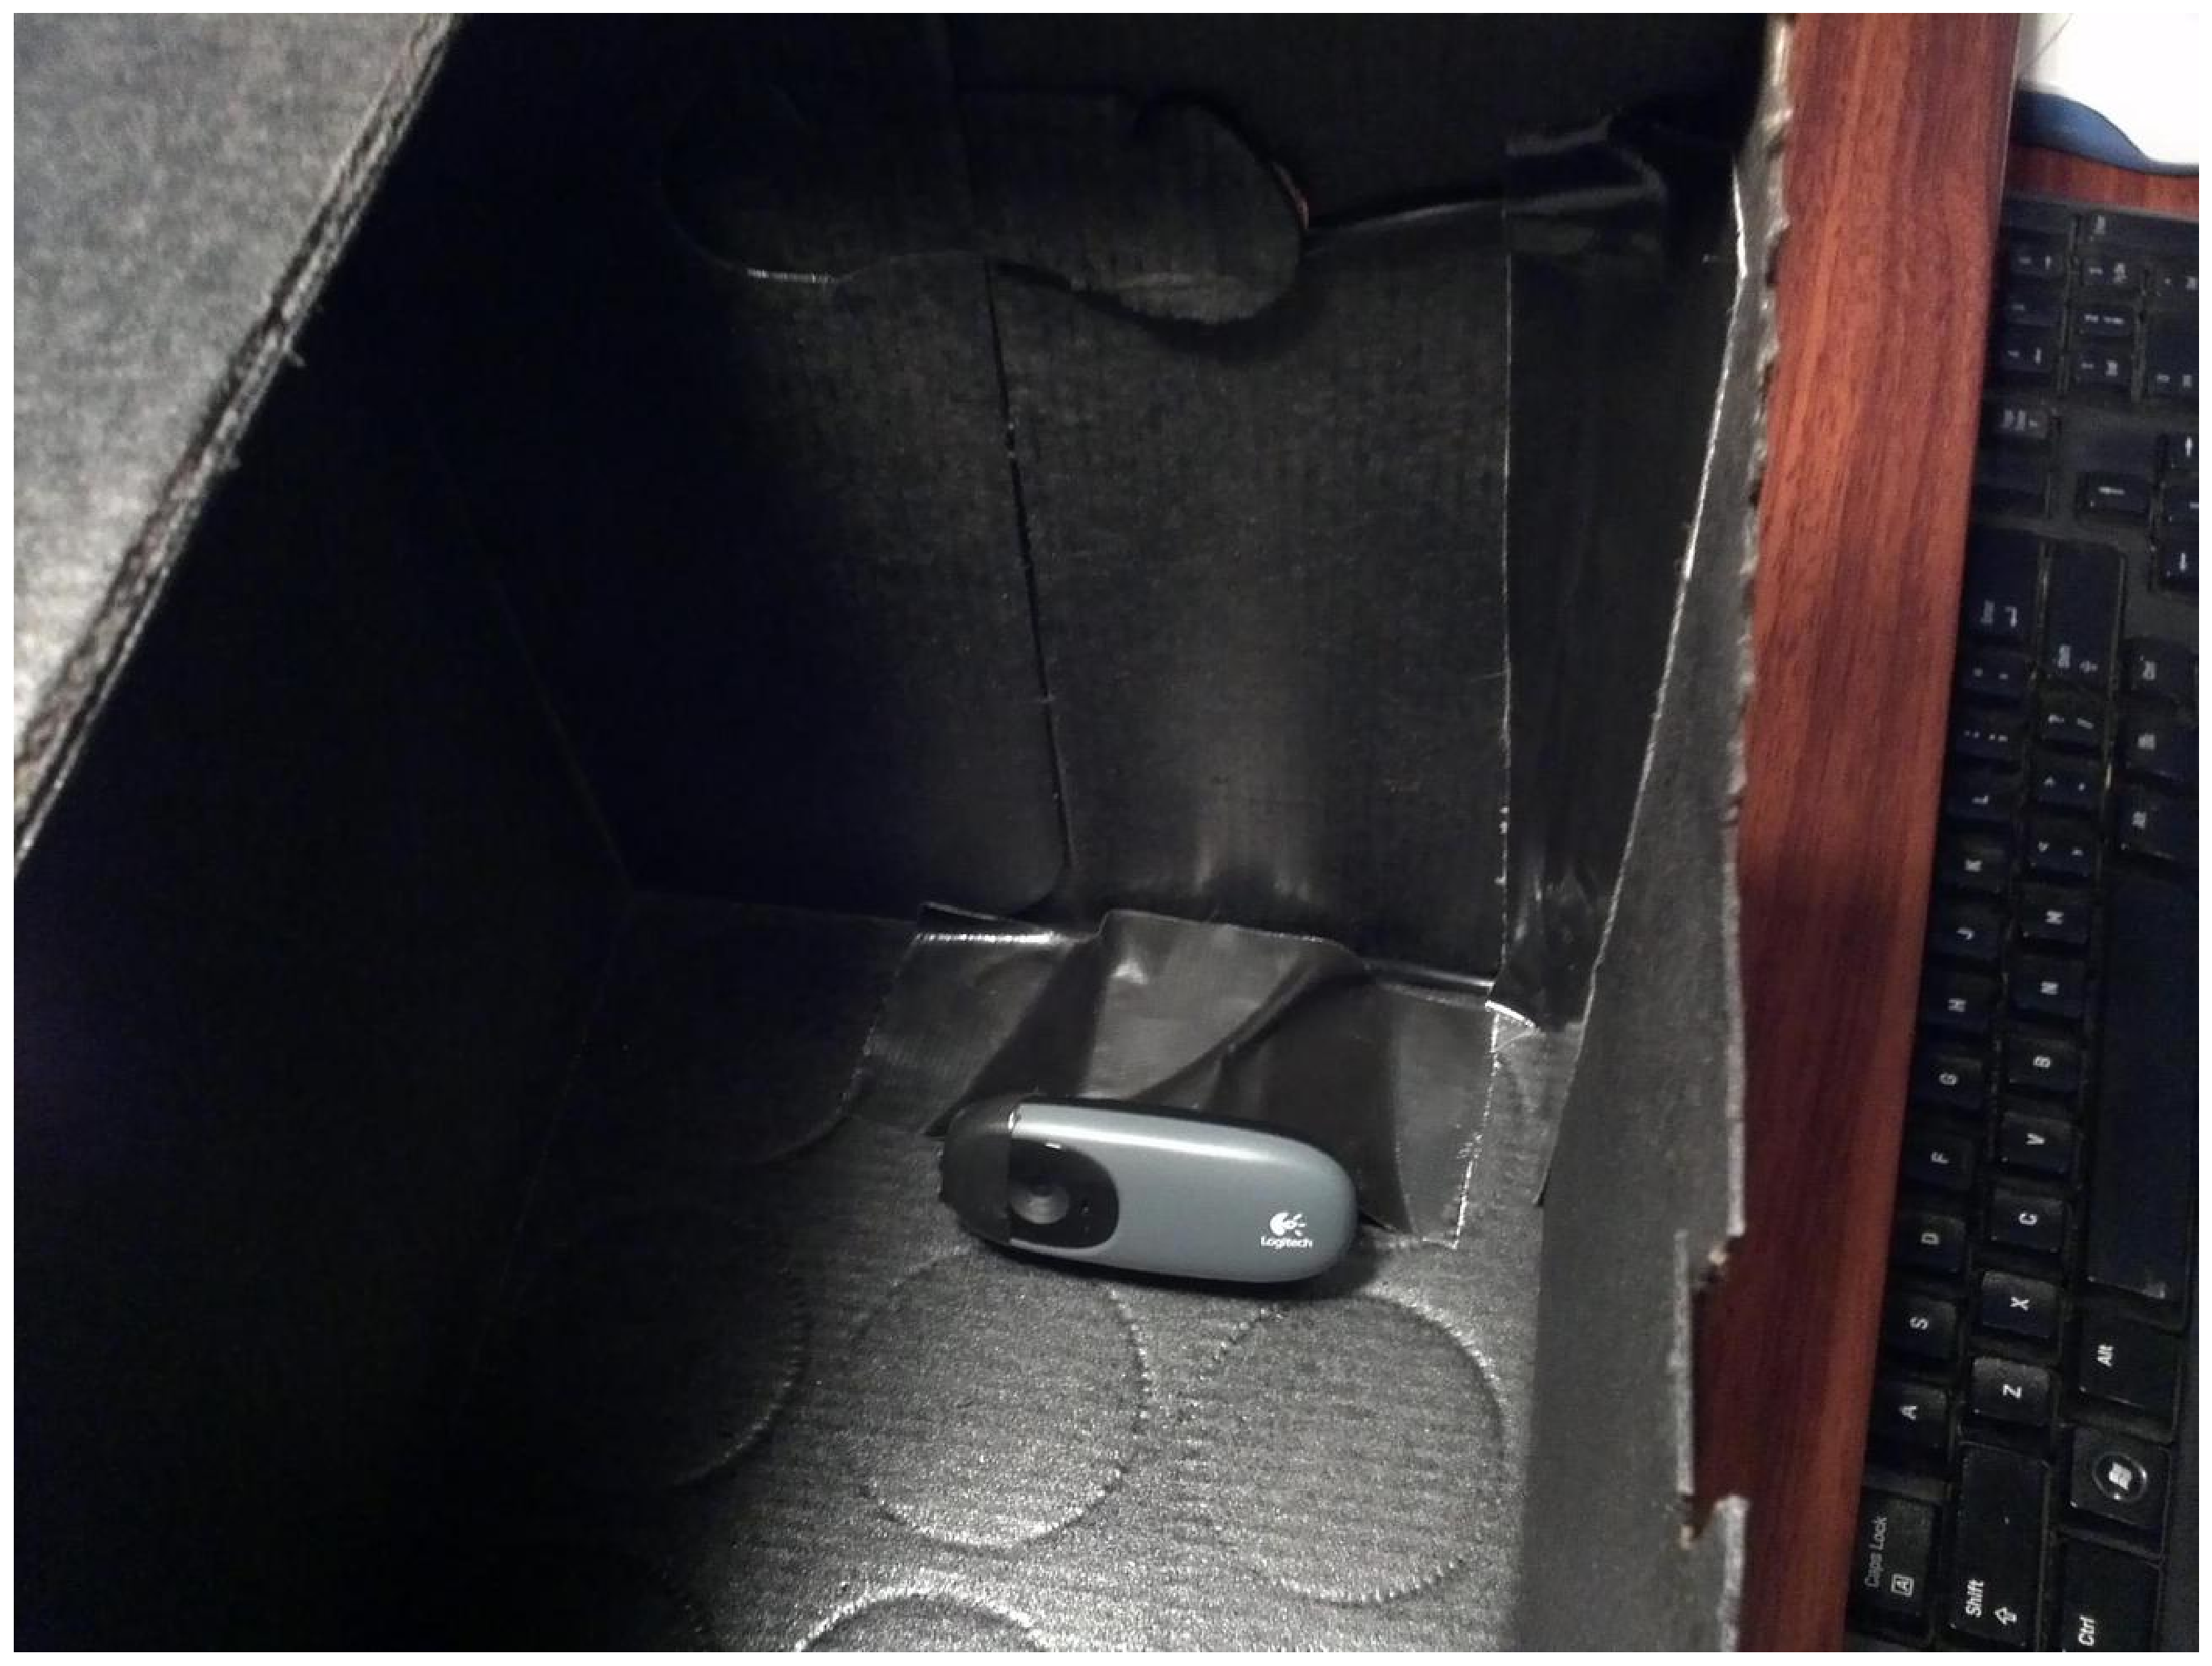
\includegraphics[width=0.8\textwidth]{eps/webcamIn.eps}
\caption{Place the webcam on the box bottom against the wall opposite of the paper stack. Hook up the webcam to a computer and use live video feed to adjust the camera angle until the white papers is fairly centered. Tape the camera and cord down when the desired viewing angle has been found.}
\end{figure}

\begin{figure}[ht!]
\centering
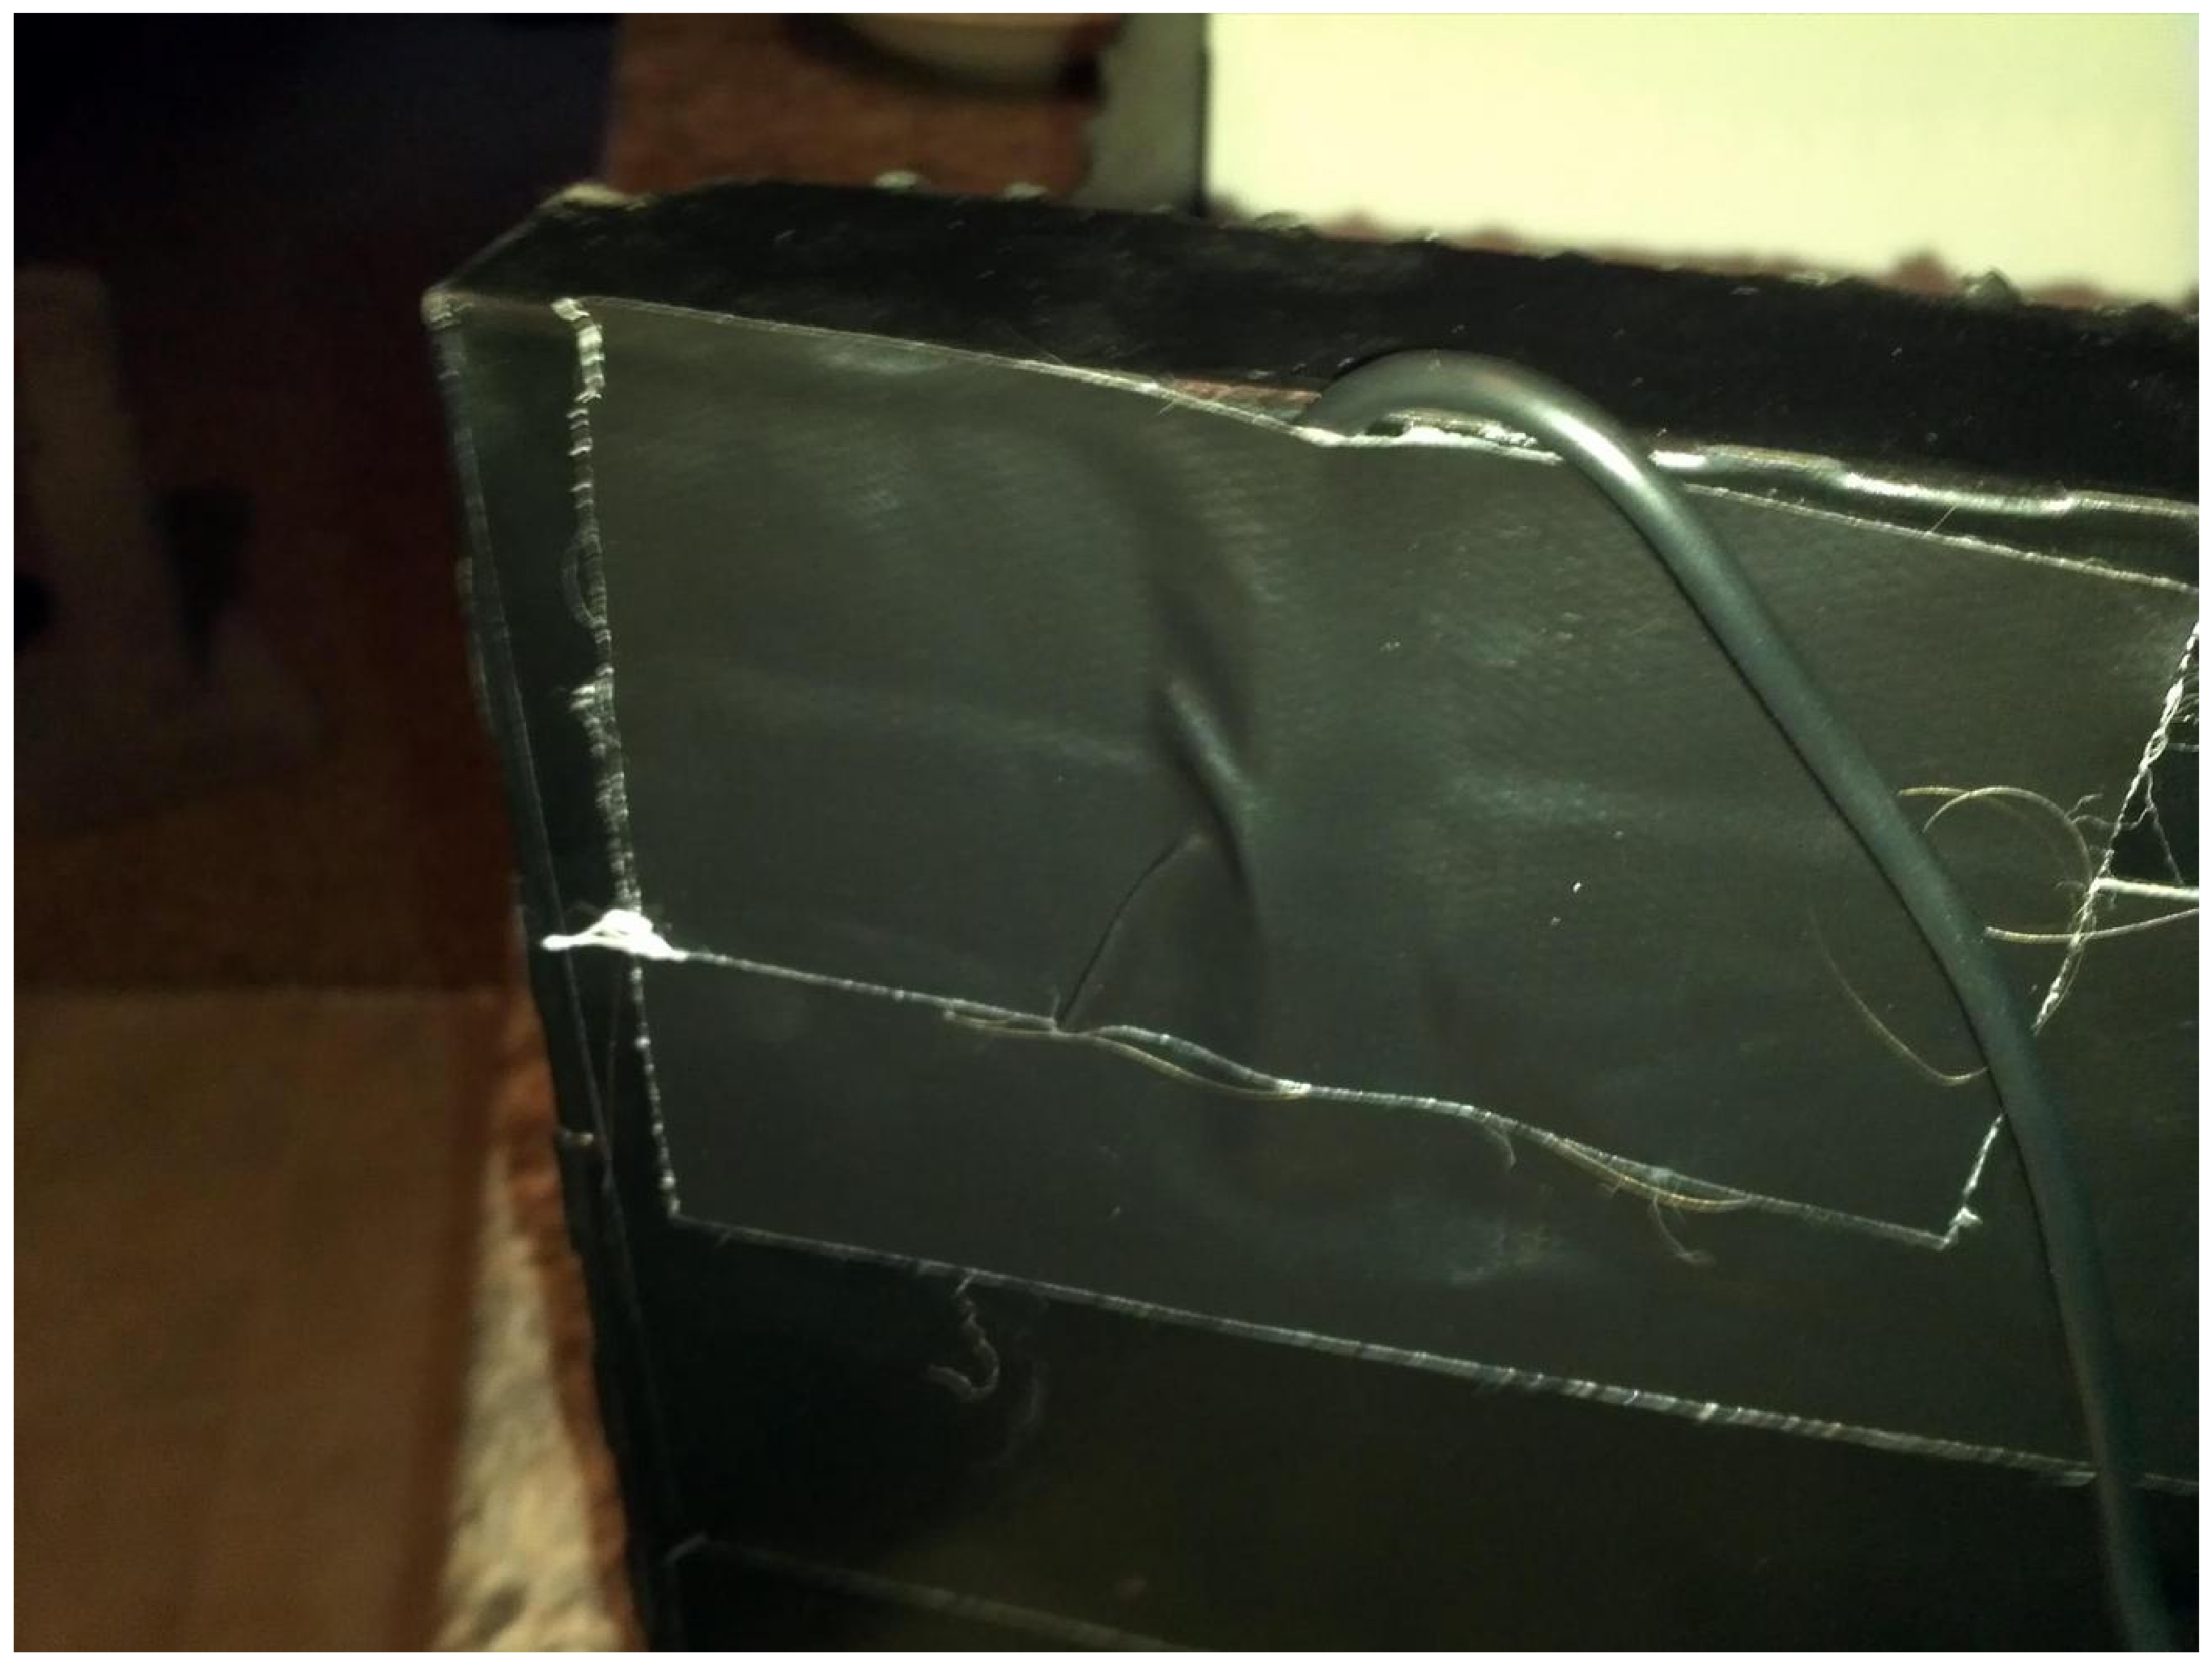
\includegraphics[width=0.8\textwidth]{eps/cordTaped.eps}
\caption{Tape the cord against the outside of the box to relieve stress if the cord is pulled.}
\end{figure}

\begin{figure}[ht!]
\centering
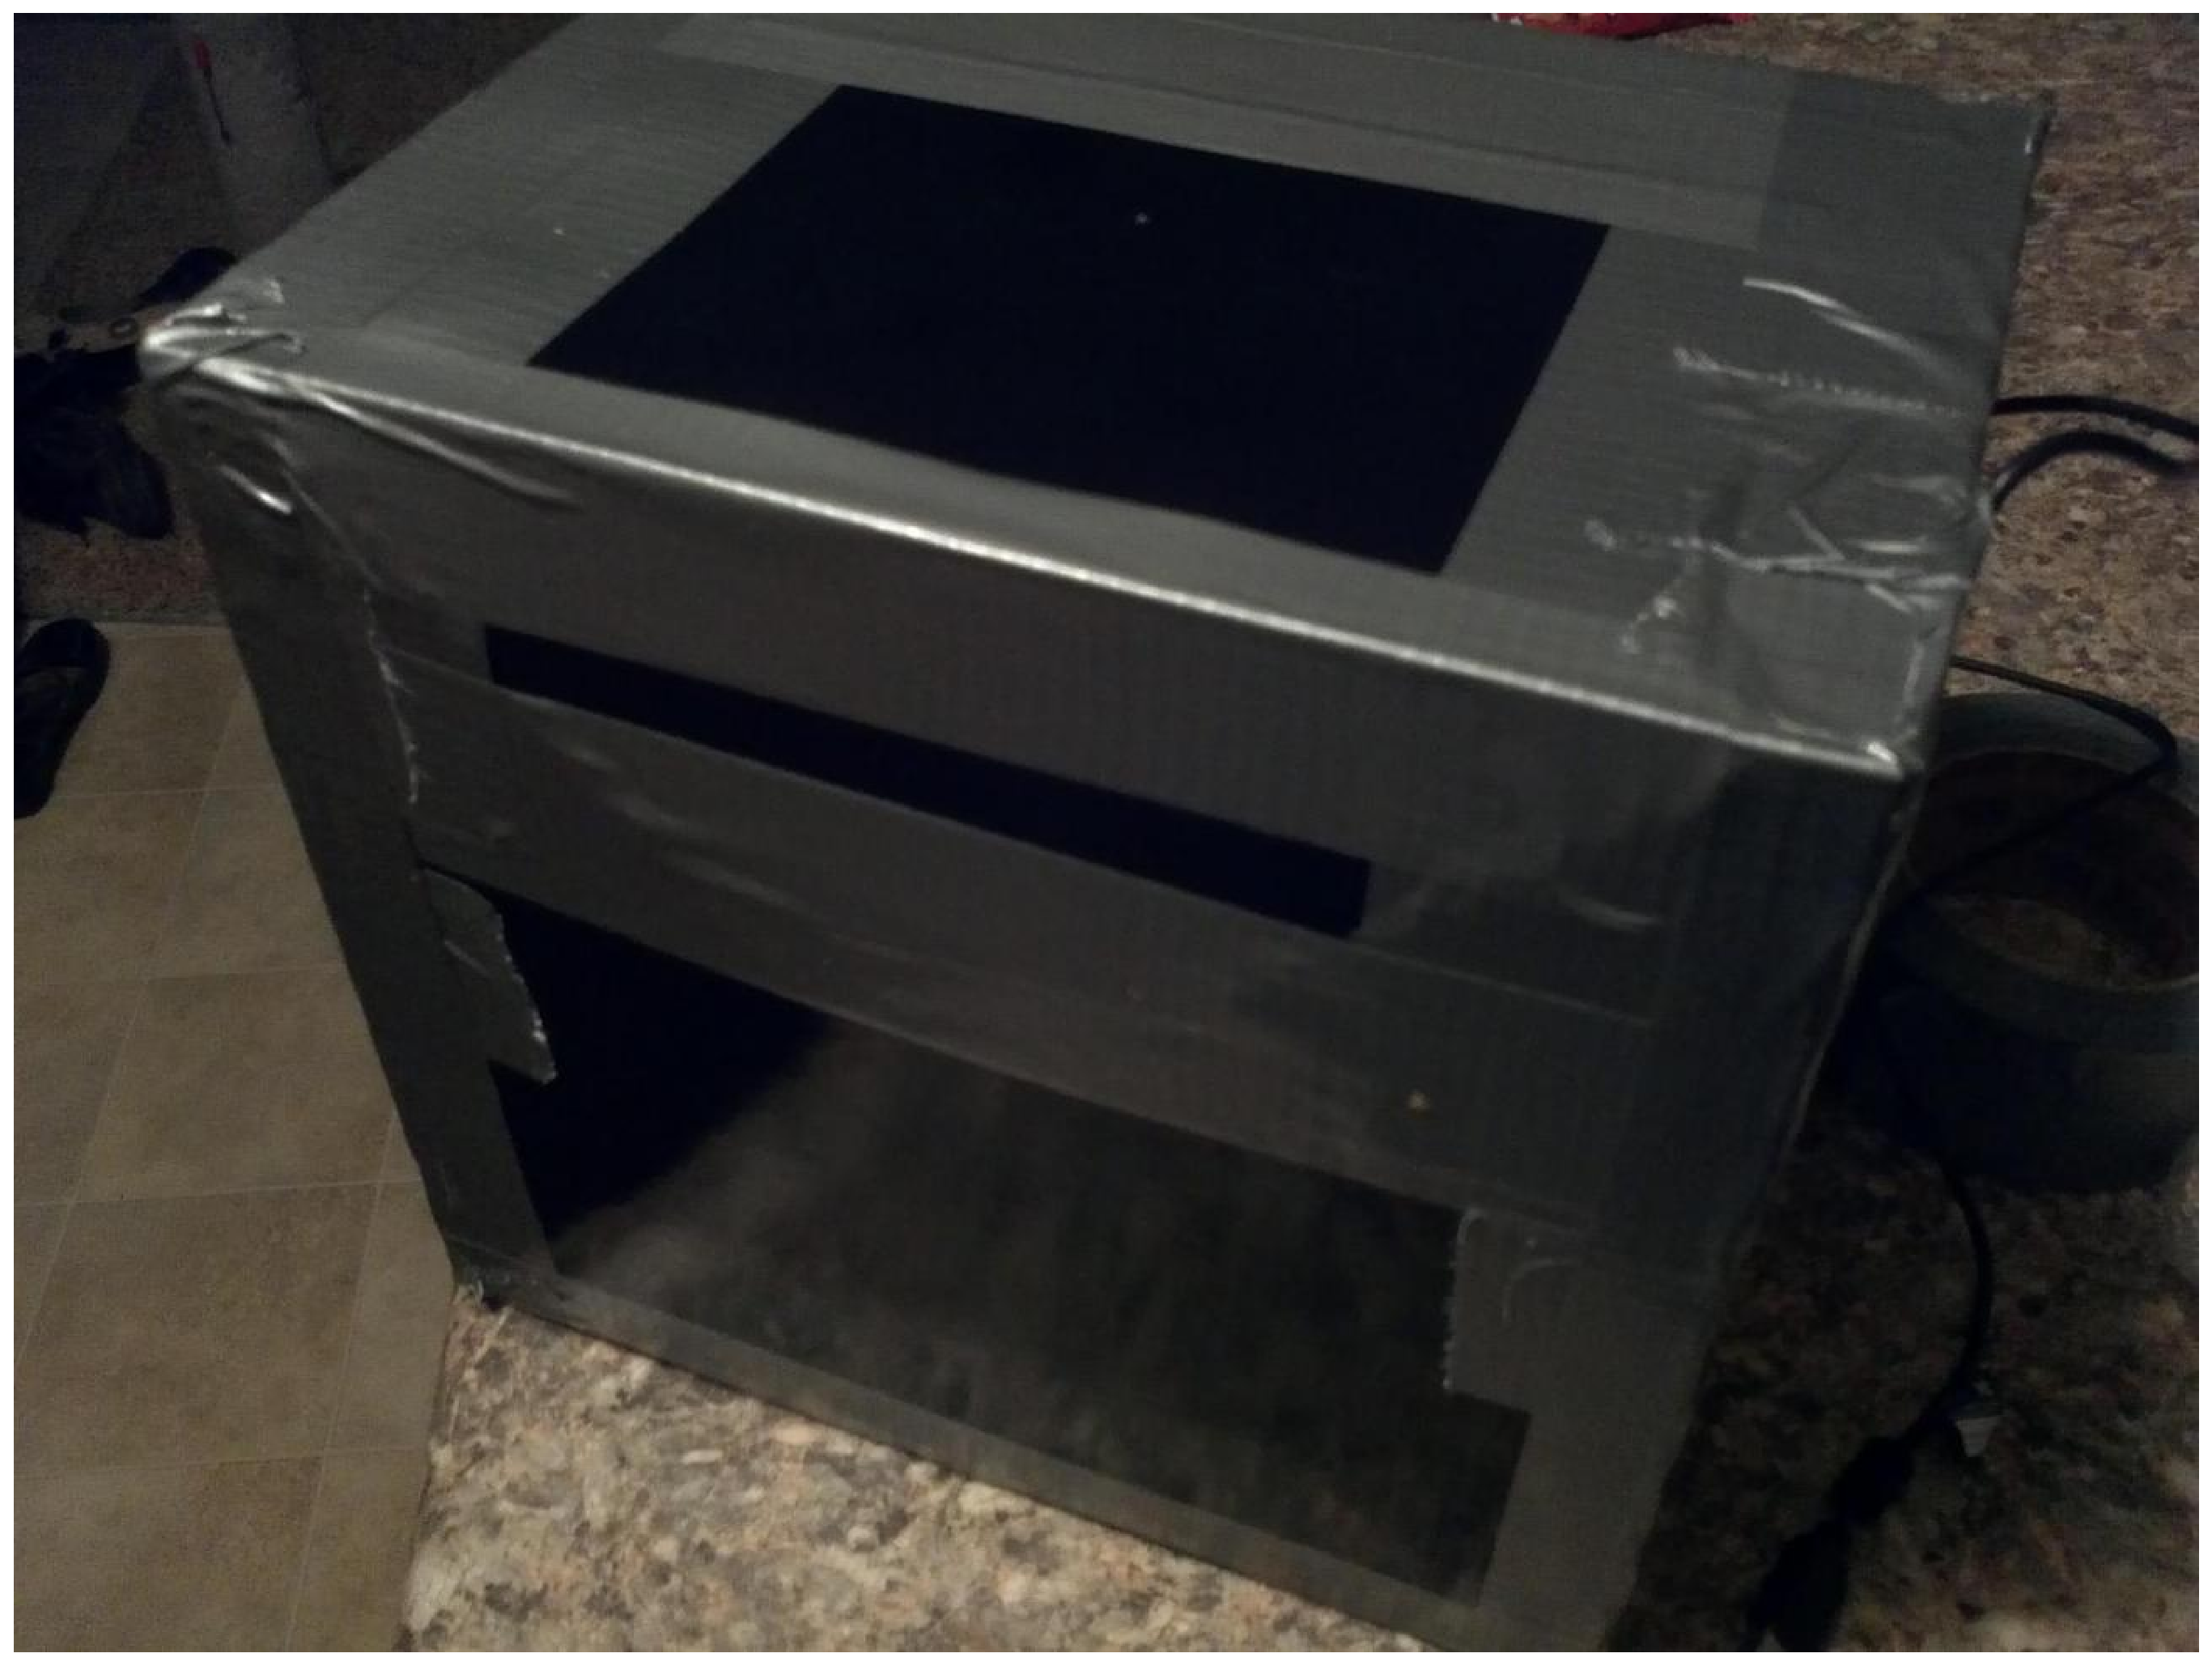
\includegraphics[width=0.8\textwidth]{eps/majorTaped.eps}
\caption{Tape up the major cracks and voids.}
\end{figure}

\begin{figure}[ht!]
\centering
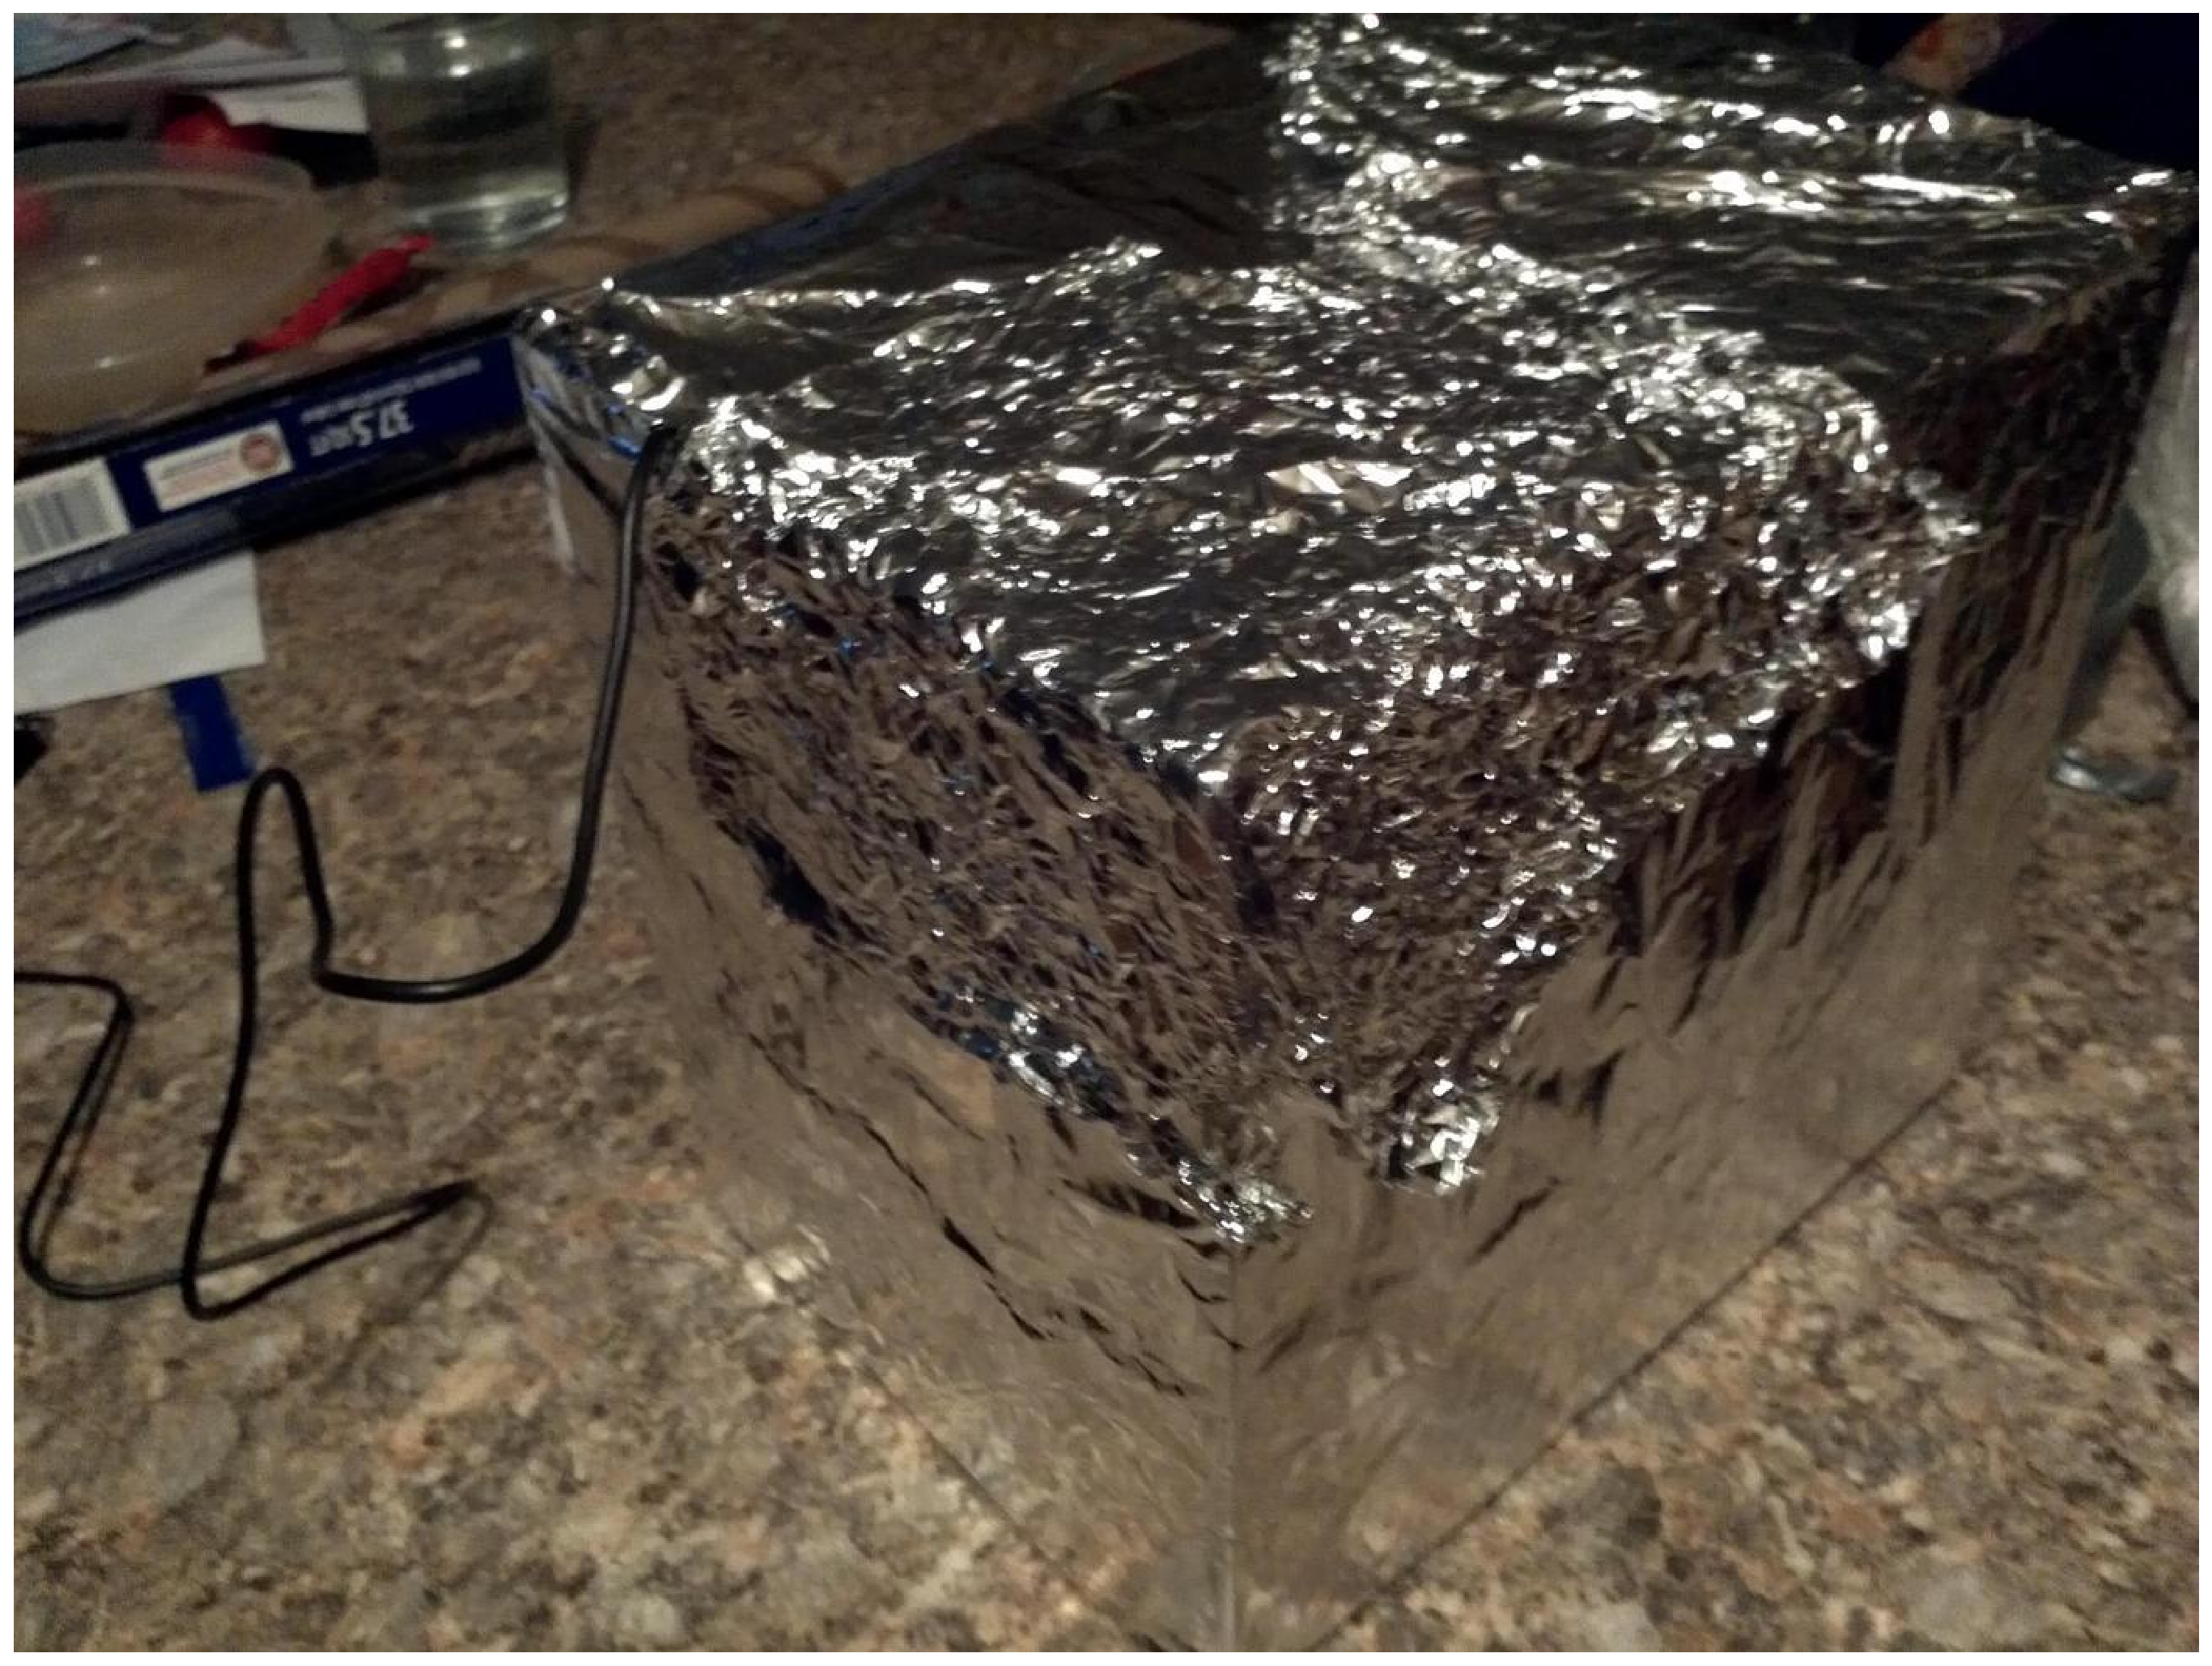
\includegraphics[width=0.8\textwidth]{eps/foilBox.eps}
\caption{Use foil to wrap the box up like a present.}
\end{figure}

\begin{figure}[ht!]
\centering
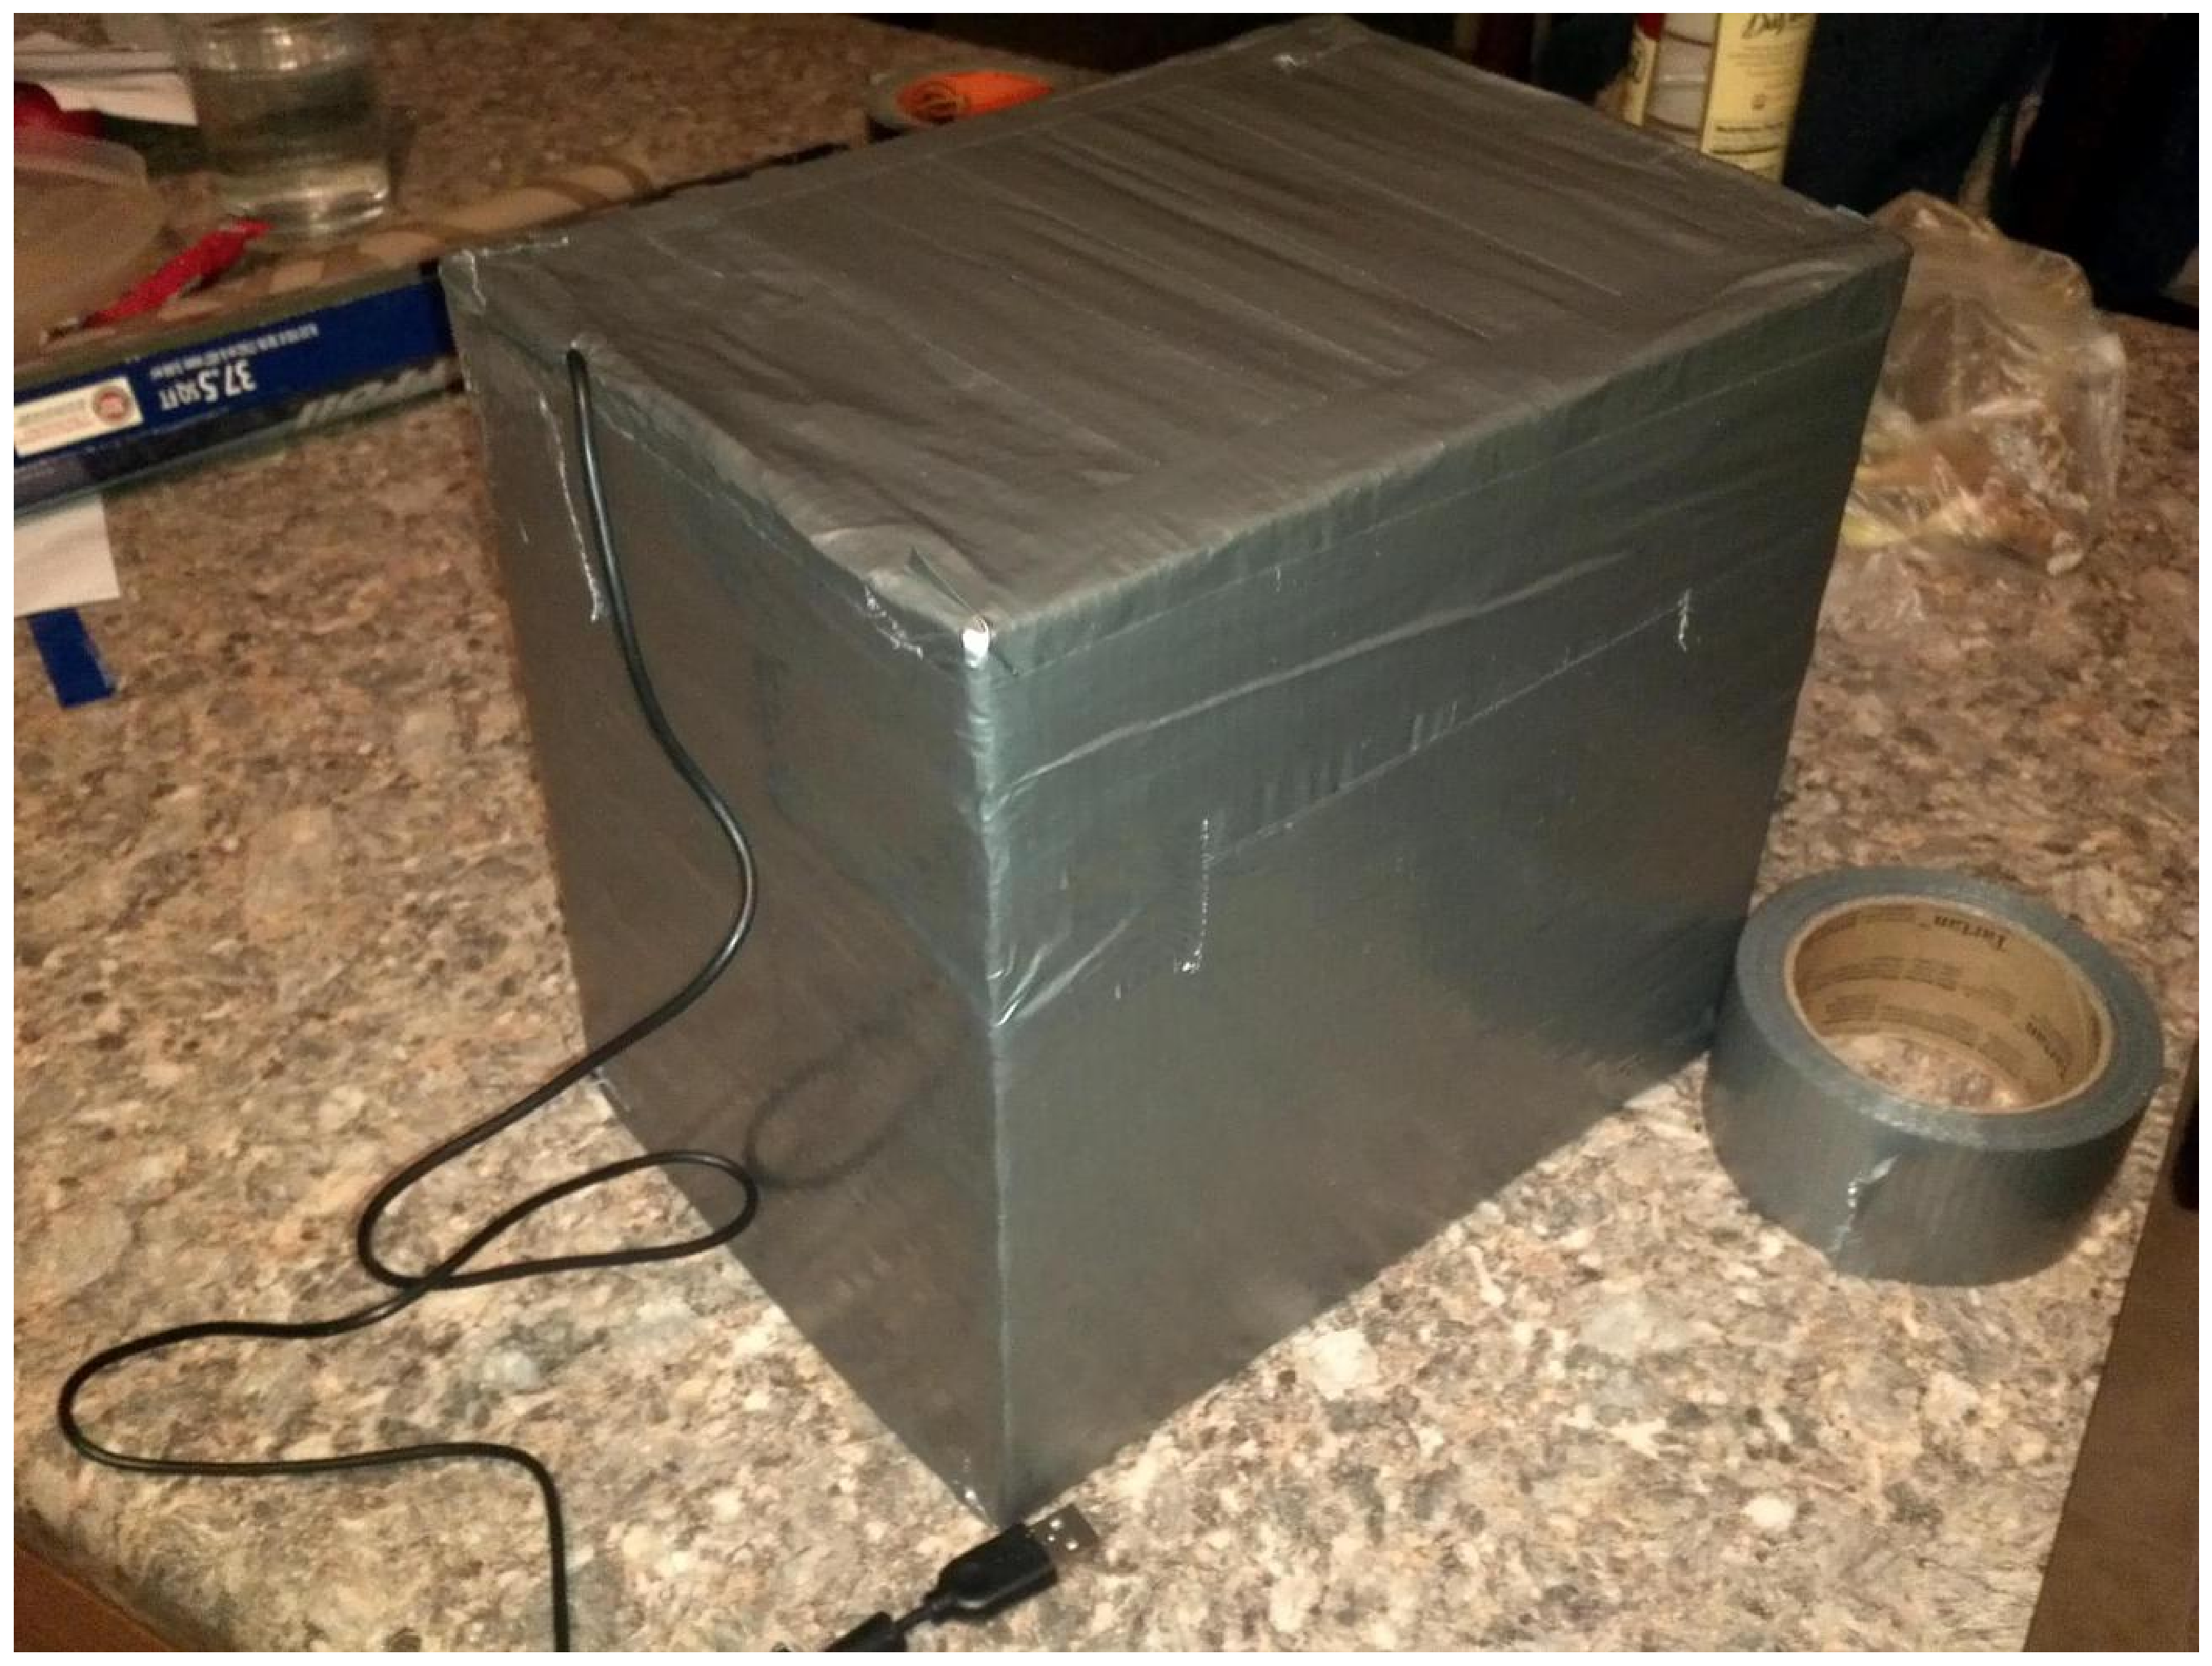
\includegraphics[width=0.8\textwidth]{eps/tapedBox.eps}
\caption{Now thoroughly tape the entire box}
\end{figure}

\begin{figure}[ht!]
\centering
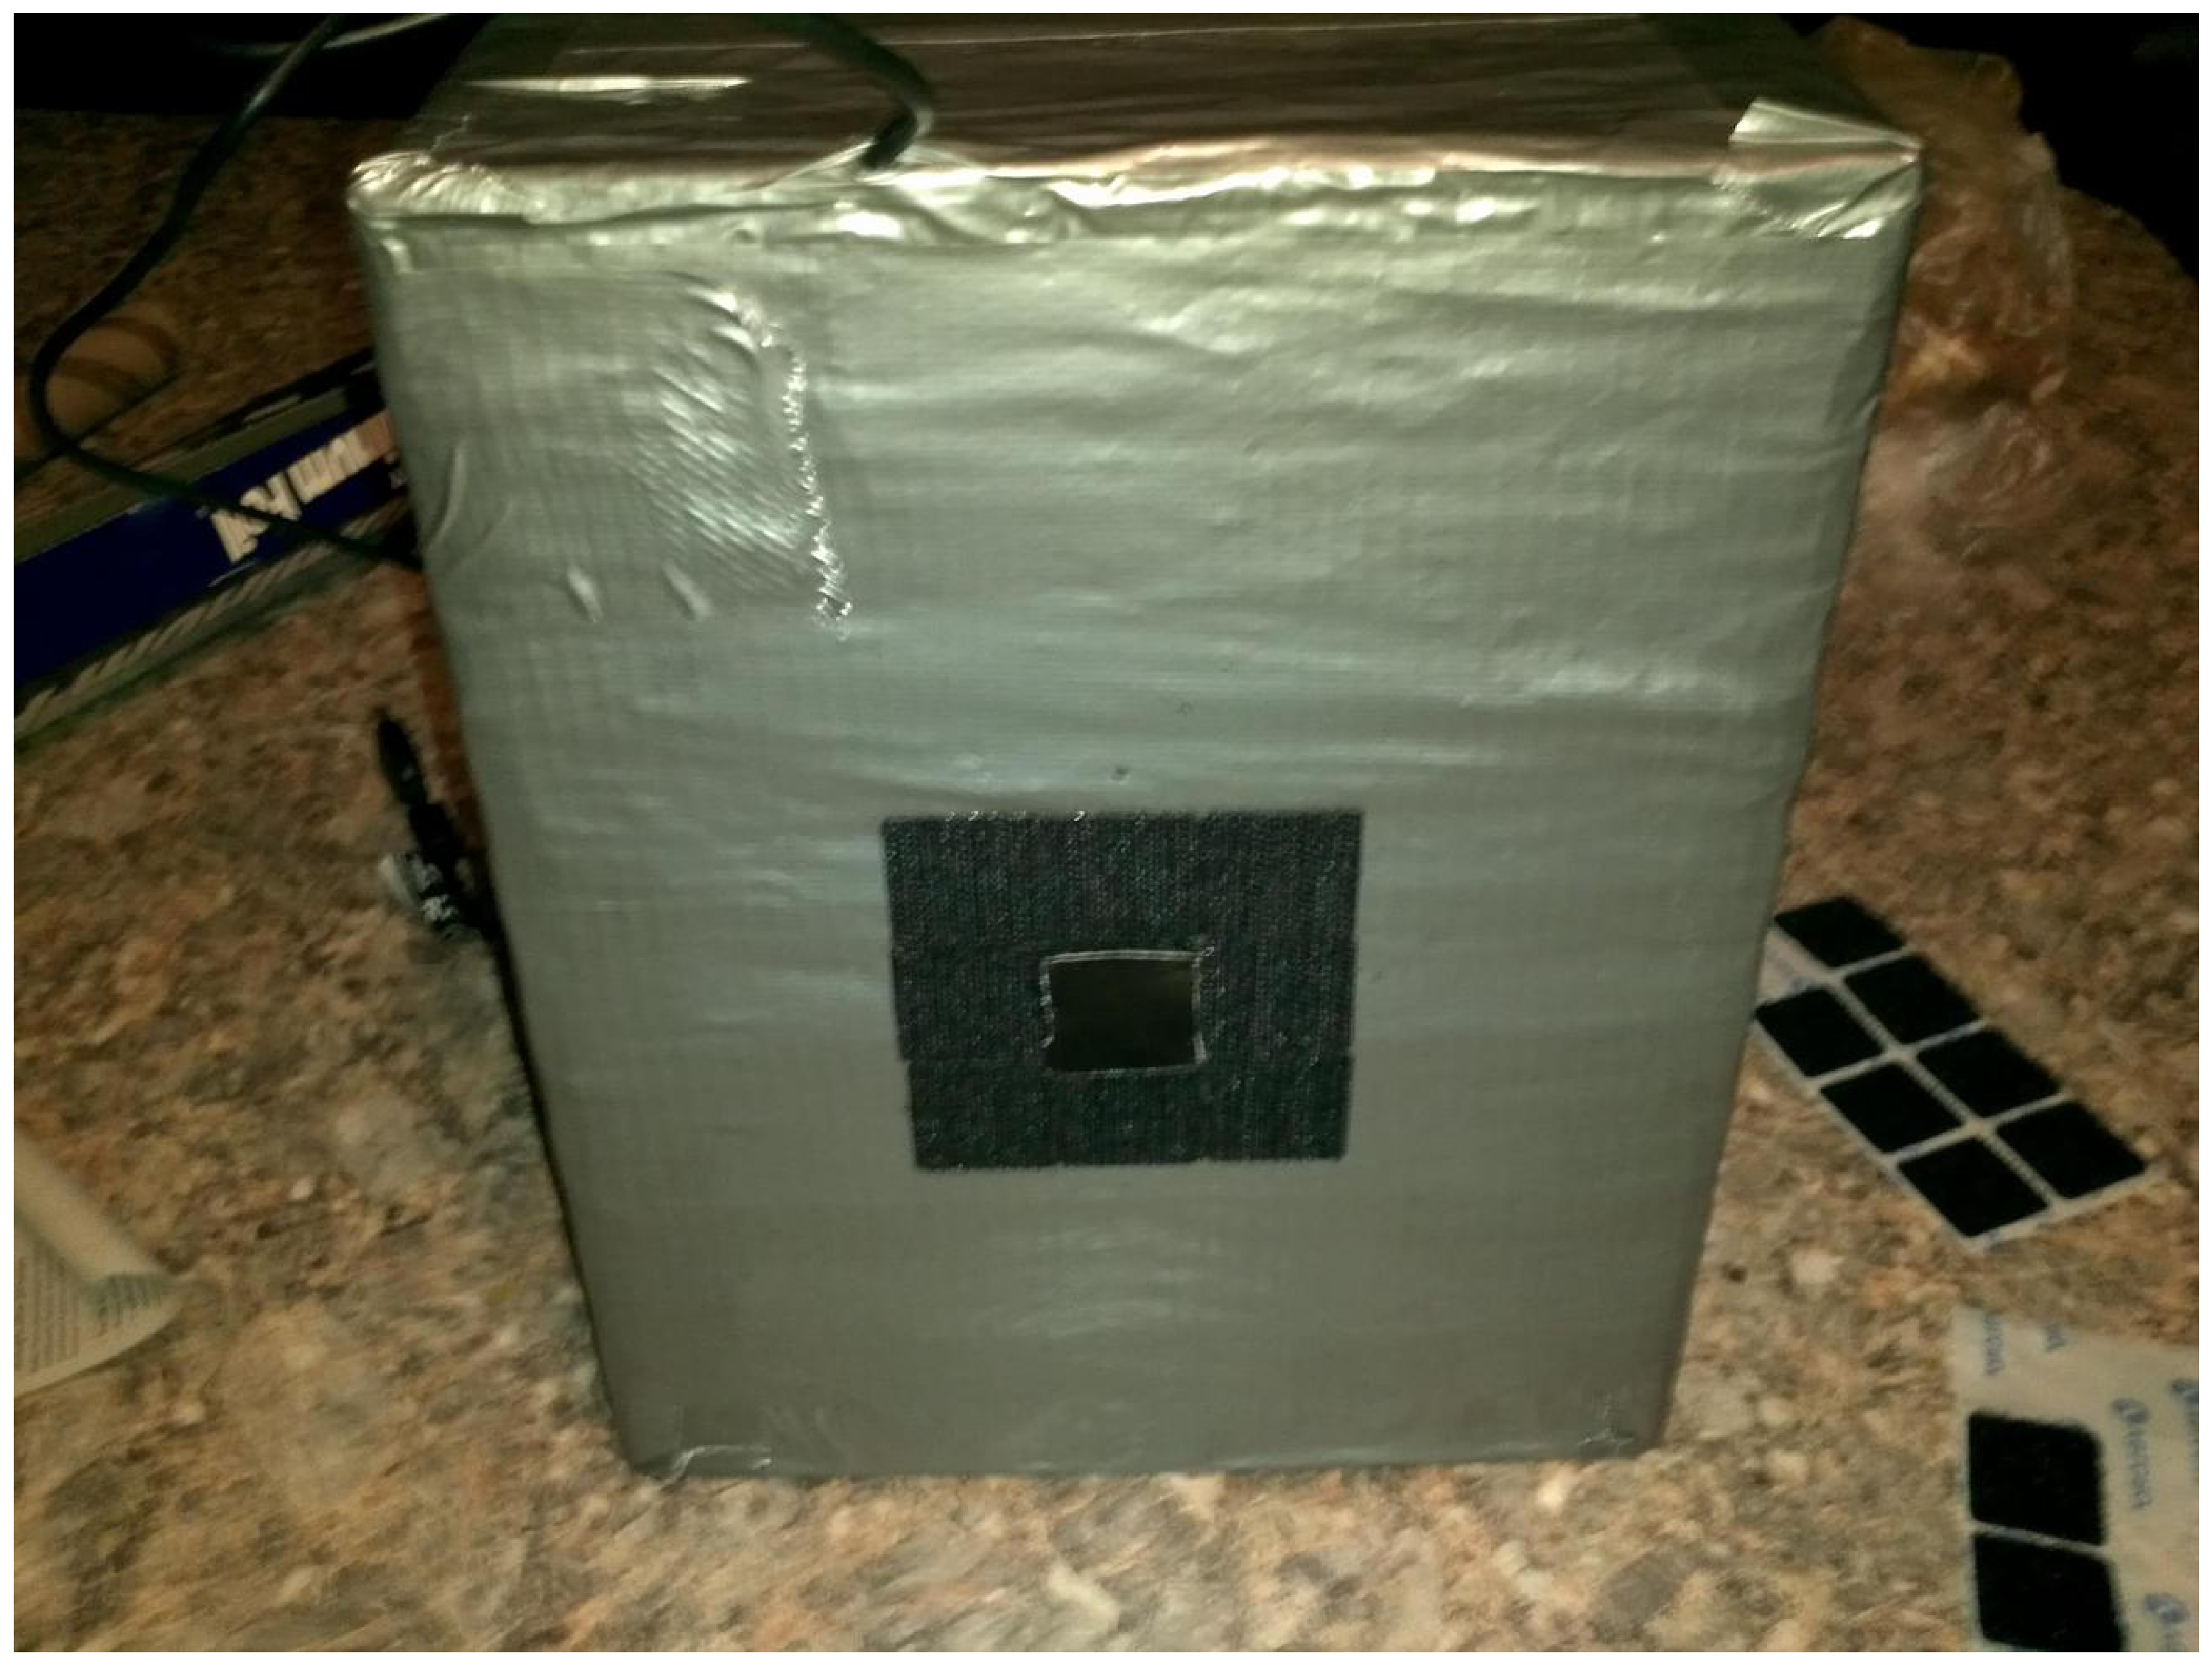
\includegraphics[width=0.8\textwidth]{eps/velcroHoles.eps}
\caption{For playing around with multiple hole sizes and positions, velcro patches are used so that the unused holes can be covered.}
\end{figure}

\begin{figure}[ht!]
\centering
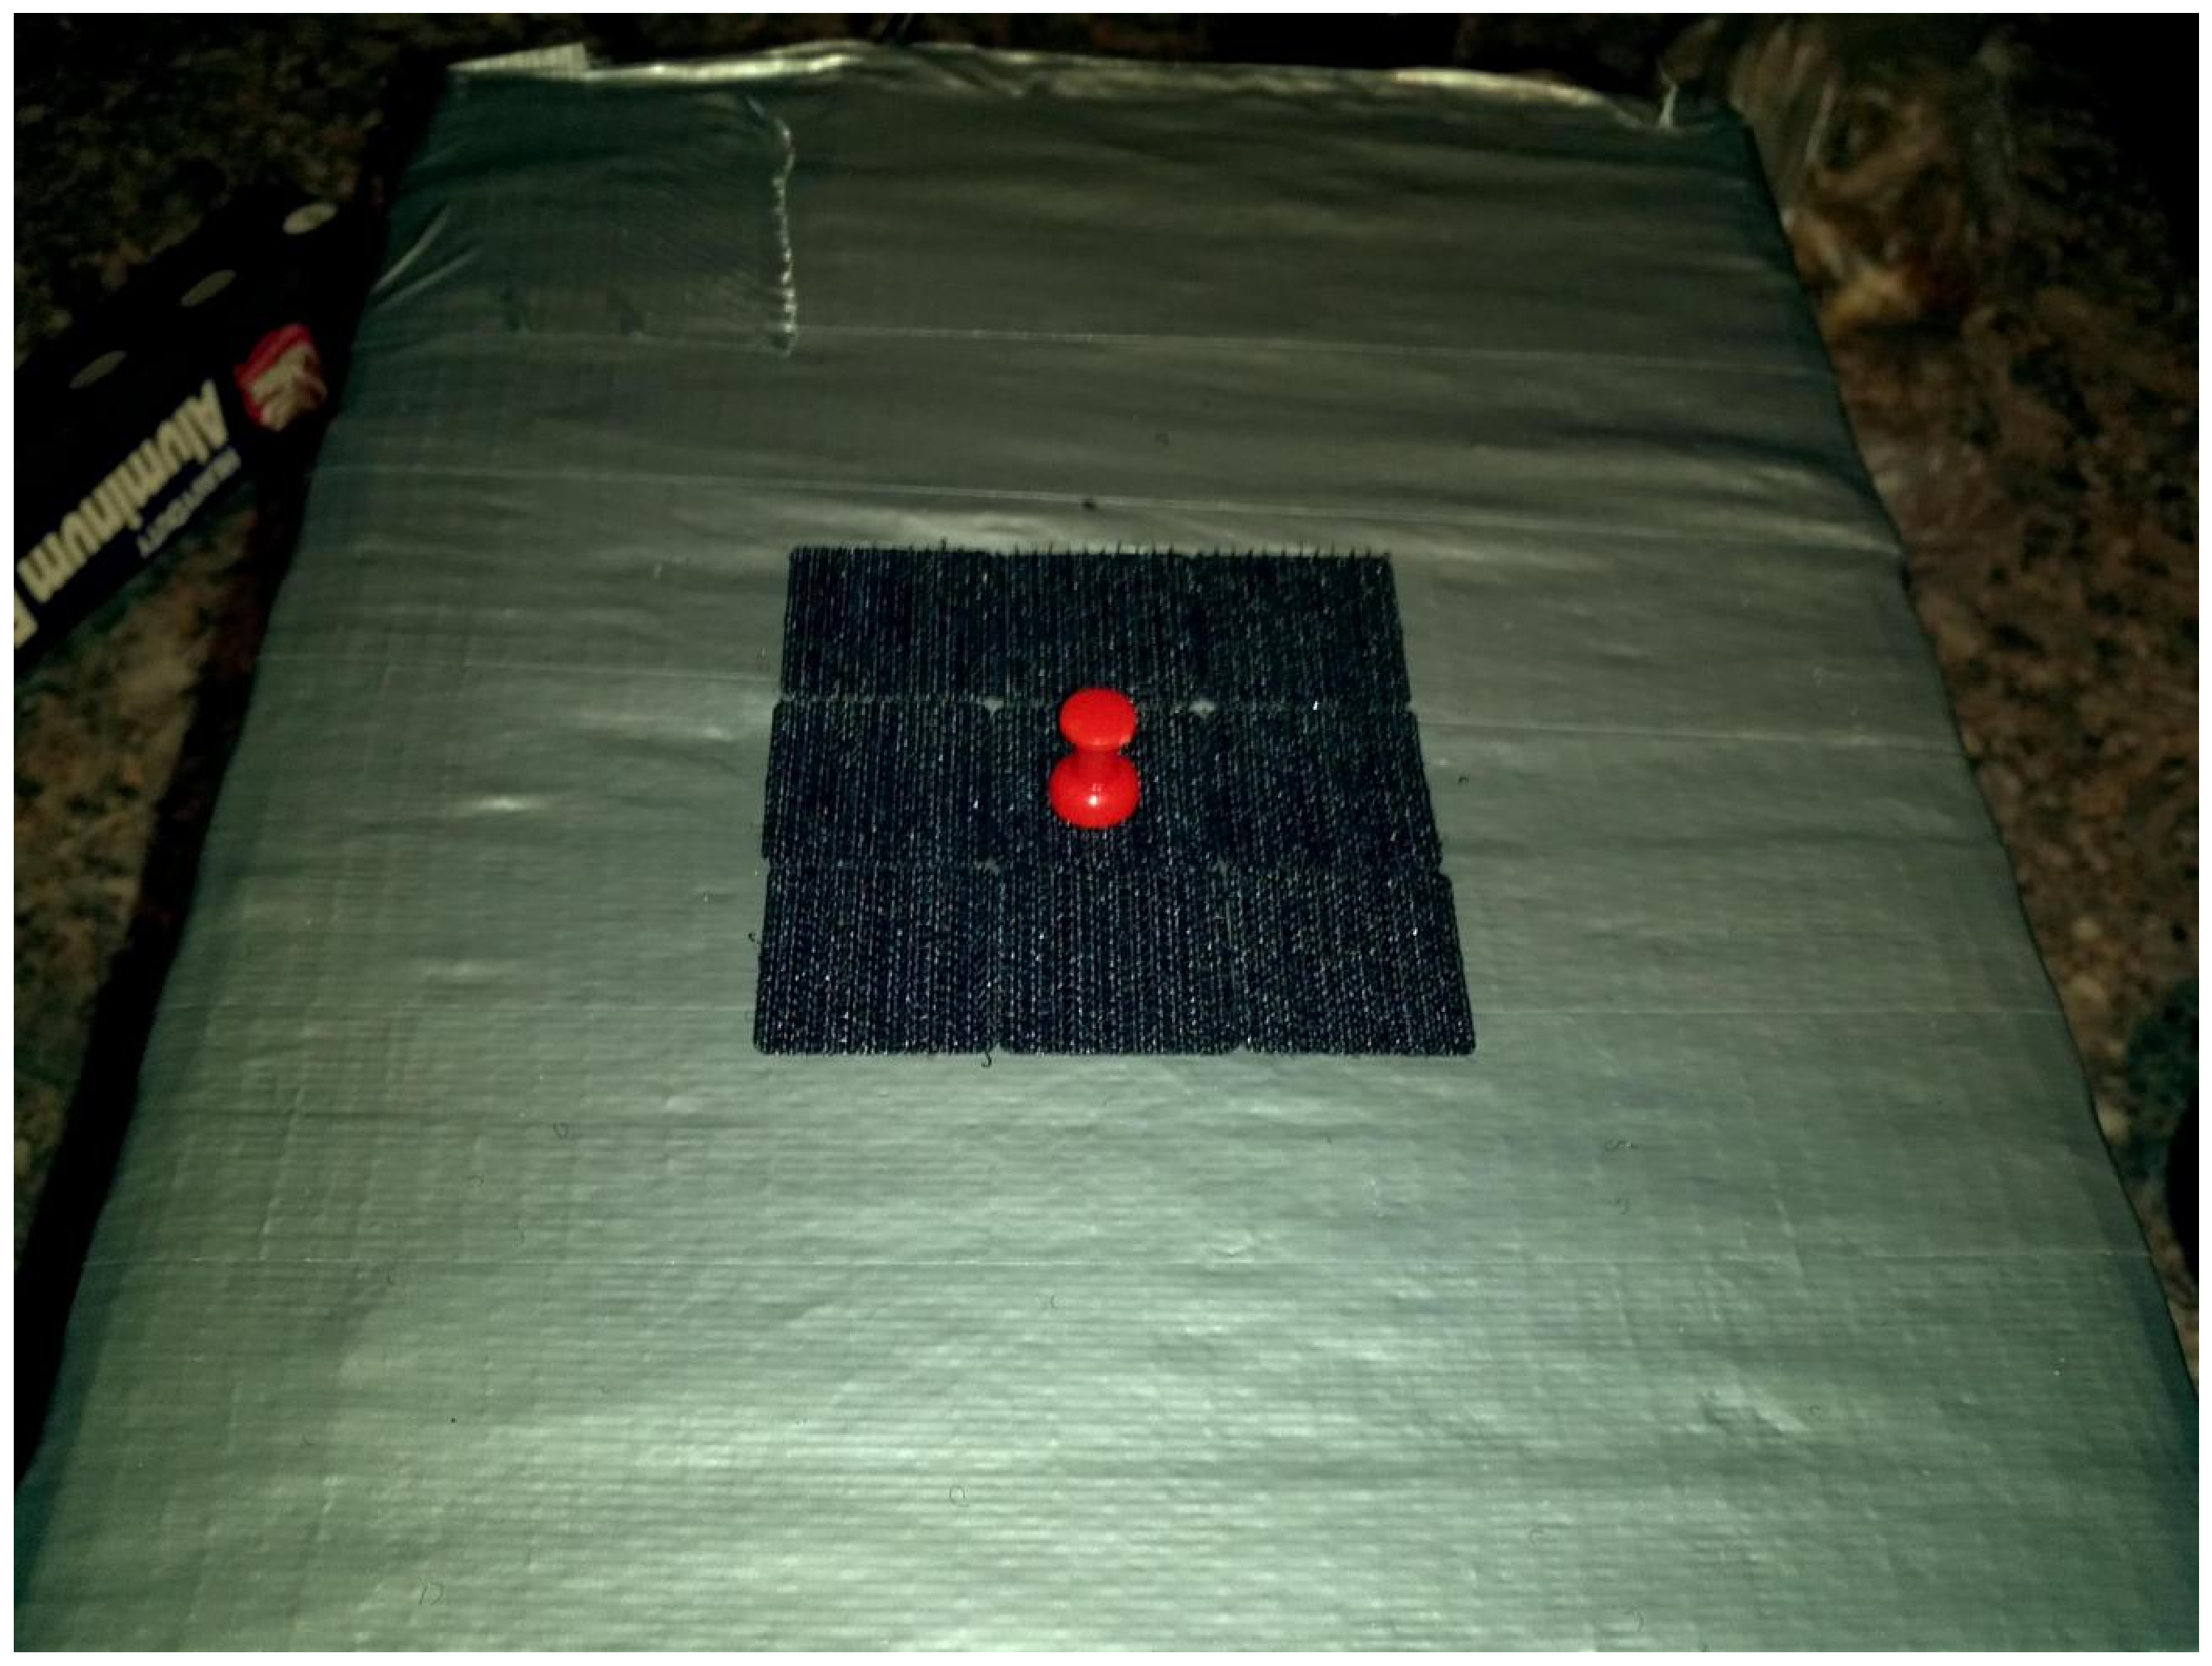
\includegraphics[width=0.8\textwidth]{eps/pinhole.eps}
\caption{The viewing hole is then made in the middle of the velcro patch. A pin was found to be too small and a drill was used which gave good results.}
\end{figure}

\end{document}